\documentclass[11pt]{article}
\usepackage[margin=1in]{geometry}
\usepackage{times}
\usepackage{hyperref}
\usepackage{booktabs}
\usepackage{graphicx}
\usepackage{amsmath}
\usepackage{amssymb}
\usepackage{xcolor}
\usepackage{enumitem}
\usepackage{fancyhdr}
\usepackage{float}
\usepackage{caption}

\hypersetup{colorlinks=true,linkcolor=black,citecolor=black,urlcolor=blue}

\newcommand{\rishiqwarning}{%
\begin{center}
\fbox{\parbox{0.92\linewidth}{\small\textbf{Working methods + discovery manuscript.}
Confirmatory H1 has \emph{not} been unlocked.
Human validation and OSF preregistration remain outstanding.
System~B discovery exhibits are exploratory under a heuristic annotator on public-domain development text.
Success is \emph{not} defined as a positive quantum result.}}
\end{center}}

\title{Beyond Metaphor:\\
\large A Blinded Confirmatory Design and Computational Discovery Engine\\
for Quantum-Structural Analogues in Classical Sanskrit Thought}
\author{RISHI-Q Project\\[0.35em]
\small Working manuscript --- methodology, instrument validation, and exploratory discovery\\
\small Local repository build}
\date{\today}

\pagestyle{fancy}
\fancyhf{}
\fancyhead[L]{\small RISHI-Q working draft}
\fancyhead[R]{\small Systems A+B; confirmatory locked}
\fancyfoot[C]{\thepage}

\begin{document}
\maketitle
\rishiqwarning

\begin{abstract}
Claims that classical Sanskrit philosophical texts ``anticipated quantum mechanics'' are culturally pervasive but scientifically fragile: once modern physics is known, ambiguous metaphysical language can be reinterpreted until it sounds quantum-like.
RISHI-Q (Research Instrument for Structural Historical Inference of Quantum-analogues) is a dual-system computational research project.
\textbf{System~A} is a preregisterable confirmatory experiment asking whether selected Sanskrit corpora exhibit \emph{quantum-specific} structural correspondence with QM/QFT beyond matched historical controls, after blinding, translation controls, vocabulary masking, evidence-constrained annotation, and cluster-aware inference.
\textbf{System~B} is a computational discovery engine that extracts evidence-bound concept graphs, mines unsupervised \emph{Rishi Motifs} \emph{without} physics labels, then maps motifs to physical theories only post hoc---searching for previously unquantified structural patterns, translation effects, anomalies, and claim--data divergences.
The framework separates Level~I (generic metaphysical), Level~II (classical/field-like), and Level~III (quantum-specific) similarity and forbids upgrading metaphors such as unity into entanglement.
This manuscript documents the scientific design, ontology, pipelines, reproducibility machinery, instrument validation on synthetic and modern-physics controls, an exploratory public-domain pilot, and System~B discovery outputs.
It does \textbf{not} claim confirmatory Sanskrit results or Tier-5 transformative discoveries.
A negative confirmatory result remains a successful scientific outcome.
\end{abstract}

\tableofcontents
\newpage

\section{Introduction}
\subsection{Motivation}
Popular and semi-scholarly literature frequently maps Sanskrit concepts---pr\={a}\d{n}a, \={a}k\={a}\'{s}a, \'sakti, Brahman, spanda, a\d{n}u/param\={a}\d{n}u---onto energy, fields, vibration, or quantum phenomena~\cite{capra1975}.
Such comparisons are historically interesting as \emph{cultural reception}, but they are poor evidence of structural correspondence unless they survive controls that make retrospective reinterpretation difficult~\cite{restivo1983}.

\subsection{Two complementary systems}
\begin{figure}[H]
\centering
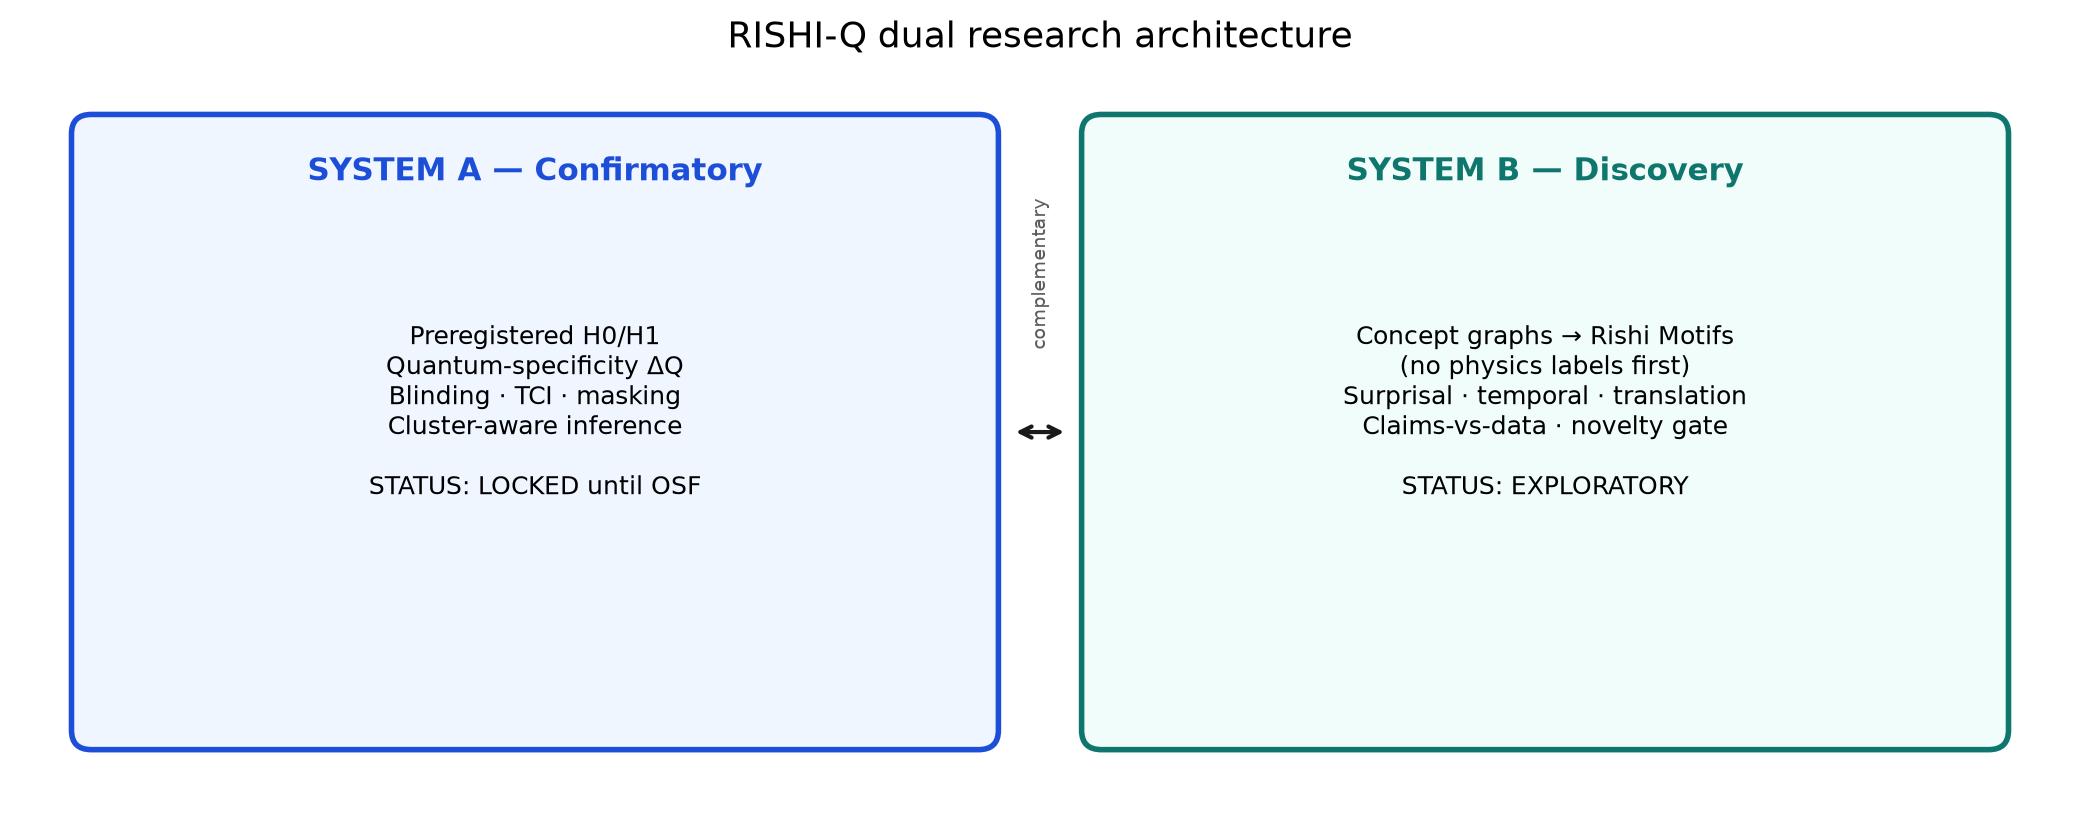
\includegraphics[width=\linewidth]{figures/fig23_dual_system.png}
\caption{RISHI-Q dual architecture: confirmatory hypothesis testing (System~A) and unsupervised structural discovery (System~B).}
\label{fig:dual}
\end{figure}
System~A preserves a sharp confirmatory question.
System~B ensures the project is not limited to confirming or rejecting an already-discussed claim: it searches for structural motifs and historical patterns that were not pre-specified as ``quantum.''

\subsection{Research questions}
\paragraph{Confirmatory (System~A).}
Do selected classical Sanskrit philosophical corpora exhibit statistically greater structural correspondence with modern QM/QFT than matched historical philosophical controls?
\paragraph{Discovery (System~B).}
Which recurring structural motifs, temporal combinations, translation shifts, anomalies, or claim--data divergences are quantitatively supported in the sampled corpora---independent of physics labels at discovery time?

\subsection{What RISHI-Q is not}
RISHI-Q is not a proof that scriptures discovered quantum mechanics; not a cosine-similarity demo between Upani\d{s}ads and physics encyclopedias; and not a spiritual affirmation project.
Even strong Level~III enrichment would establish at most a controlled structural analogy, not historical discovery.

\subsection{Design principle}
The experiment must be capable of producing a convincing negative result.
Methodological choices made \emph{only} to make Sanskrit look more quantum-like are forbidden (\texttt{protocol/decisions.md}).
Success is not defined as a positive quantum result; it is defined by rigorous search and honest reporting, including original negative or claim-contradicting findings.

\section{Related Work}
\subsection{Philosophy of quantum theory}
Level~III definitions follow contemporary philosophy of QM/QFT rather than popular slogans~\cite{lewis2016,maudlin2019,wallace2012,ruetsche2011,weinberg1995qft}.

\subsection{Classical Indian ontologies}
Atomism, substance, transformation, and substrate language in Vai\'se\d{s}ika, S\={a}\d{m}khya, and related schools must be read historically~\cite{halbfass1992,potter1977,larson1987}.

\subsection{Physics--mysticism critique}
Uncontrolled parallelisms are a known sociological pattern~\cite{restivo1983,capra1975}.
Capra-style analogy is treated as a methodological anti-pattern.

\subsection{Computational annotation}
LLM annotation can shift label distributions; human audit is mandatory (status: \textbf{REQUIRES\_EXTERNAL\_HUMAN\_VALIDATION}).

\section{Conceptual Framework}
\subsection{Three levels of similarity}
\begin{figure}[H]
\centering
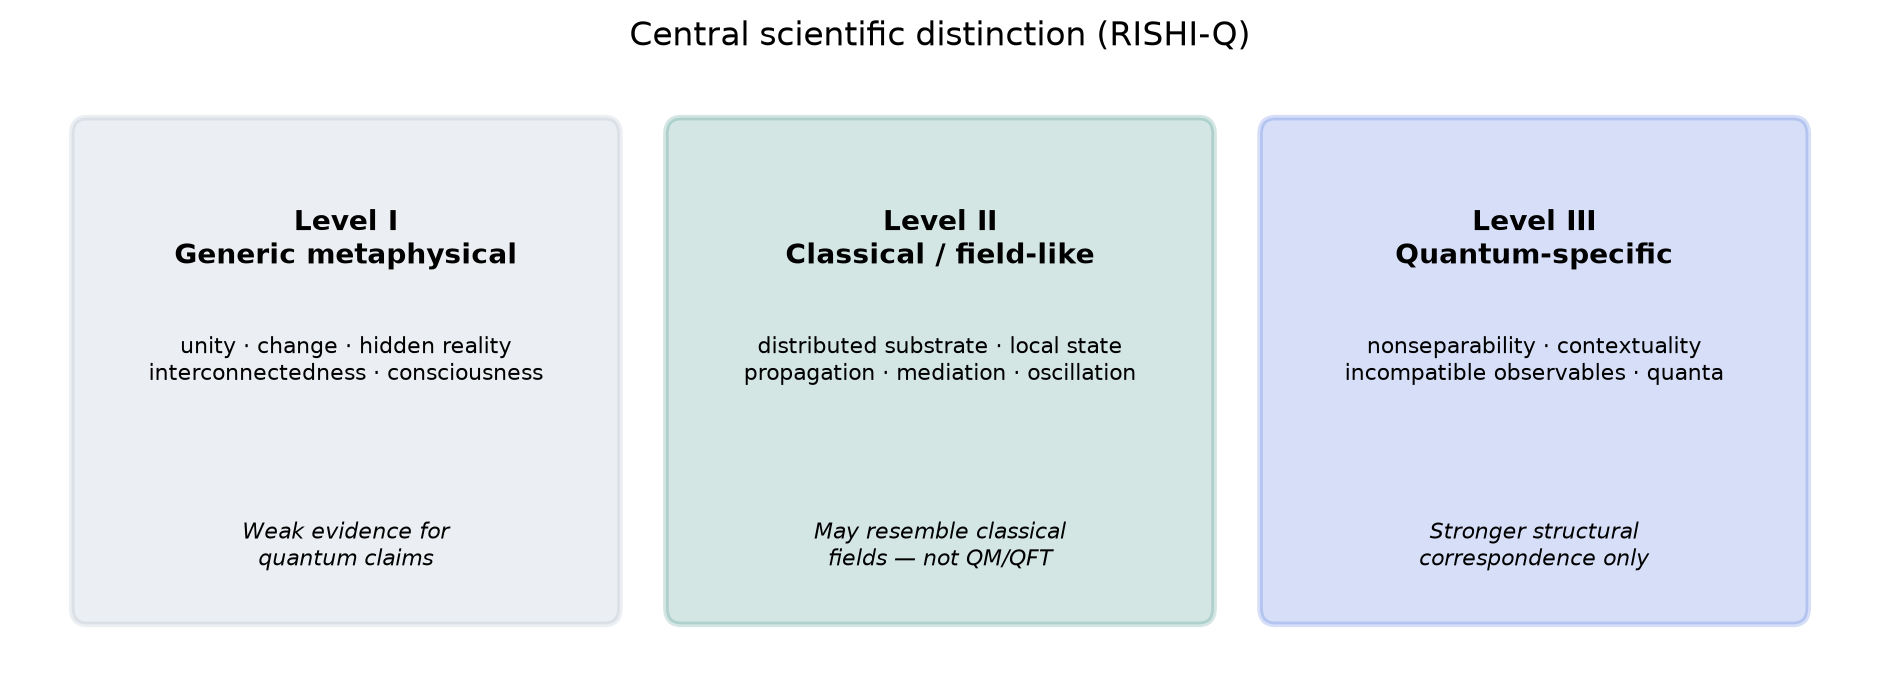
\includegraphics[width=\linewidth]{figures/fig02_three_levels.png}
\caption{Central scientific distinction: Level~I vs Level~II vs Level~III.}
\label{fig:levels}
\end{figure}
\begin{itemize}[leftmargin=*]
\item \textbf{Level I --- Generic metaphysical:} unity, change, hidden reality, interconnectedness. Weak for quantum claims.
\item \textbf{Level II --- Classical / field-like:} distributed substrate, local state, propagation, oscillation, mediation. May resemble classical fields~\cite{jackson1999}, not automatically quantum.
\item \textbf{Level III --- Quantum-specific:} discrete allowed states, fundamental probability, nonseparability, contextuality, incompatible observables, measurement-conditioned outcomes, quantized excitations.
\end{itemize}

\subsection{Hard interpretation rules}
Unity $\neq$ entanglement; vibration $\neq$ QFT; pr\={a}\d{n}a $\neq$ energy; \={a}k\={a}\'{s}a $\neq$ quantum field; a\d{n}u $\neq$ elementary particle; observer importance $\neq$ quantum measurement.
When ambiguous, prefer \texttt{NA}/\texttt{U} over \texttt{1}.
% Auto-generated — do not edit by hand
% Generated: 2026-08-15T18:05:51.960634+00:00
\begin{table}[t]
\centering
\caption{Hard interpretation rules (annotation codebook).}
\label{tab:hard-rules}
\begin{tabular}{ll}
\toprule
rule\_id & rule \\
\midrule
R01 & Everything is one does NOT imply entanglement (Q06). \\
R02 & Interconnected does NOT imply nonlocality. \\
R03 & Vibration does NOT imply QFT. \\
R04 & Prana does NOT automatically mean physical energy. \\
R05 & Akasa does NOT automatically mean a physical/quantum field. \\
R06 & Sakti does NOT automatically mean physics energy. \\
R07 & Anu does NOT automatically mean elementary particle. \\
R08 & Observer importance does NOT imply quantum measurement. \\
R09 & Epistemic uncertainty does NOT imply quantum indeterminacy. \\
R10 & Invisible does NOT imply quantum. \\
R11 & When ambiguous, prefer NA/U over 1. \\
R12 & Positive labels require exact evidence spans. \\
\bottomrule
\end{tabular}
\end{table}


\subsection{Discovery success tiers}
\begin{figure}[H]
\centering
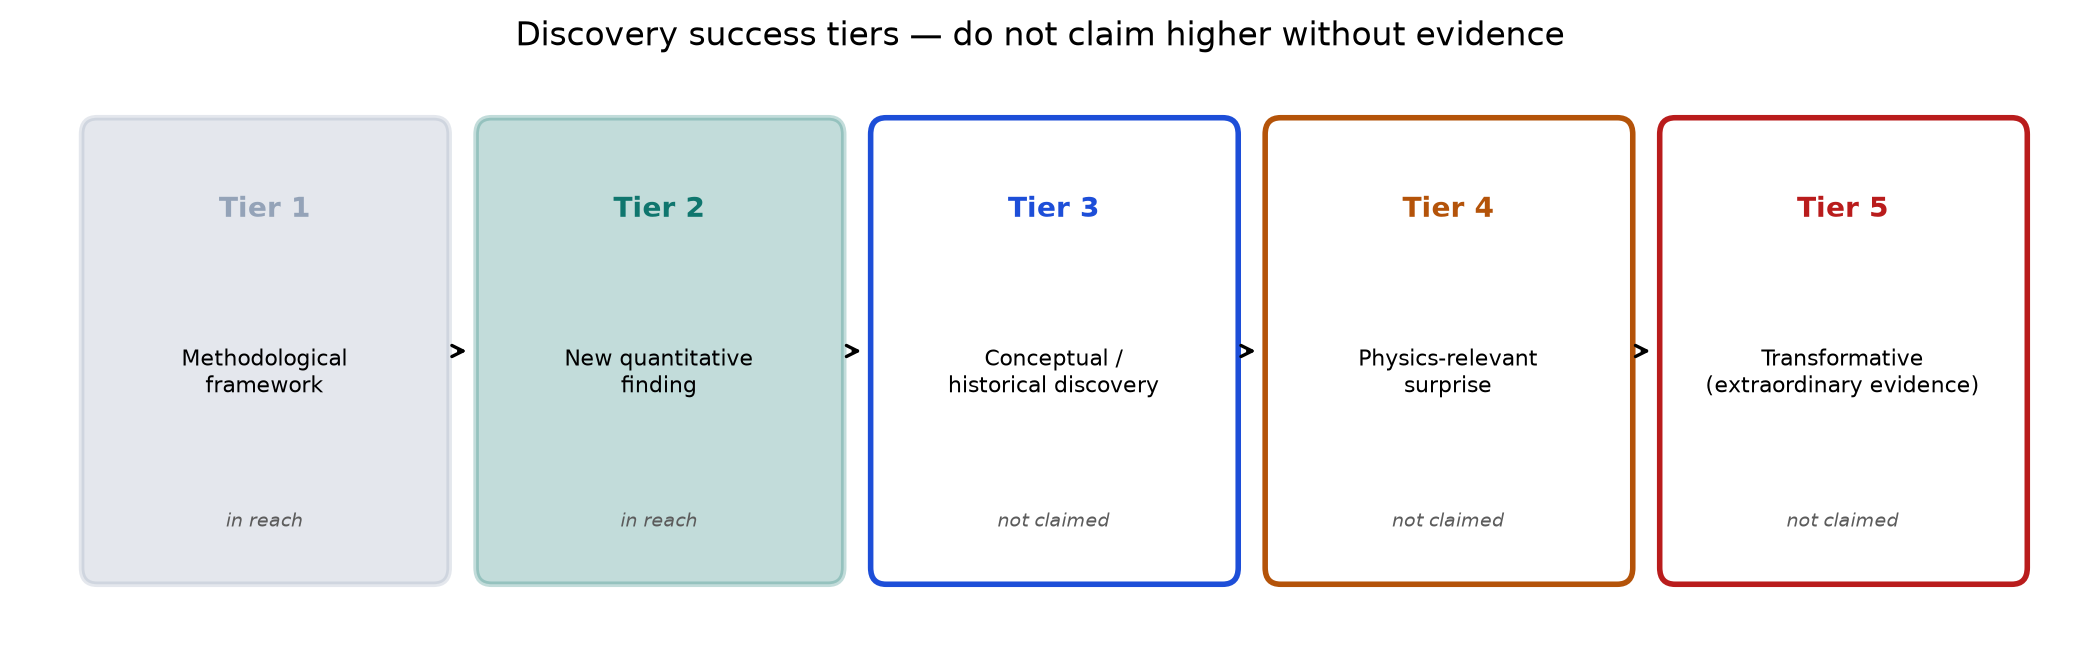
\includegraphics[width=\linewidth]{figures/fig26_success_tiers.png}
\caption{Tiered discovery success. Higher tiers require stronger evidence; Tier~5 is extraordinary.}
\label{fig:tiers}
\end{figure}

\section{Hypotheses (System~A) and Discovery Goals (System~B)}
Primary confirmatory hypotheses:
\[
H_0:\Delta_Q\le 0,\qquad H_1:\Delta_Q>0,
\]
\[
QS_i=S(X_i,Q)-\max_{C\in\mathrm{Classical}}S(X_i,C),
\quad
\Delta_Q=\mathbb{E}[QS_{\mathrm{target}}]-\mathbb{E}[QS_{\mathrm{control}}].
\]
Secondary hypotheses H2--H8 cover specificity and robustness (\texttt{protocol/hypotheses.md}).
Discovery goals D1--D8 cover motif mining, enrichment, surprisal, temporal analysis, translation shifts, claims-vs-data, atlas construction, and novelty gating---explicitly exploratory until frozen and replicated.

\section{Corpora and Firewall}
Targets: Upani\d{s}adic/Ved\={a}ntic and related schools.
Controls: Buddhist, Greek, Chinese, and other historical philosophical slices; literary negatives; modern physics references for instrument checks.
\begin{figure}[H]
\centering
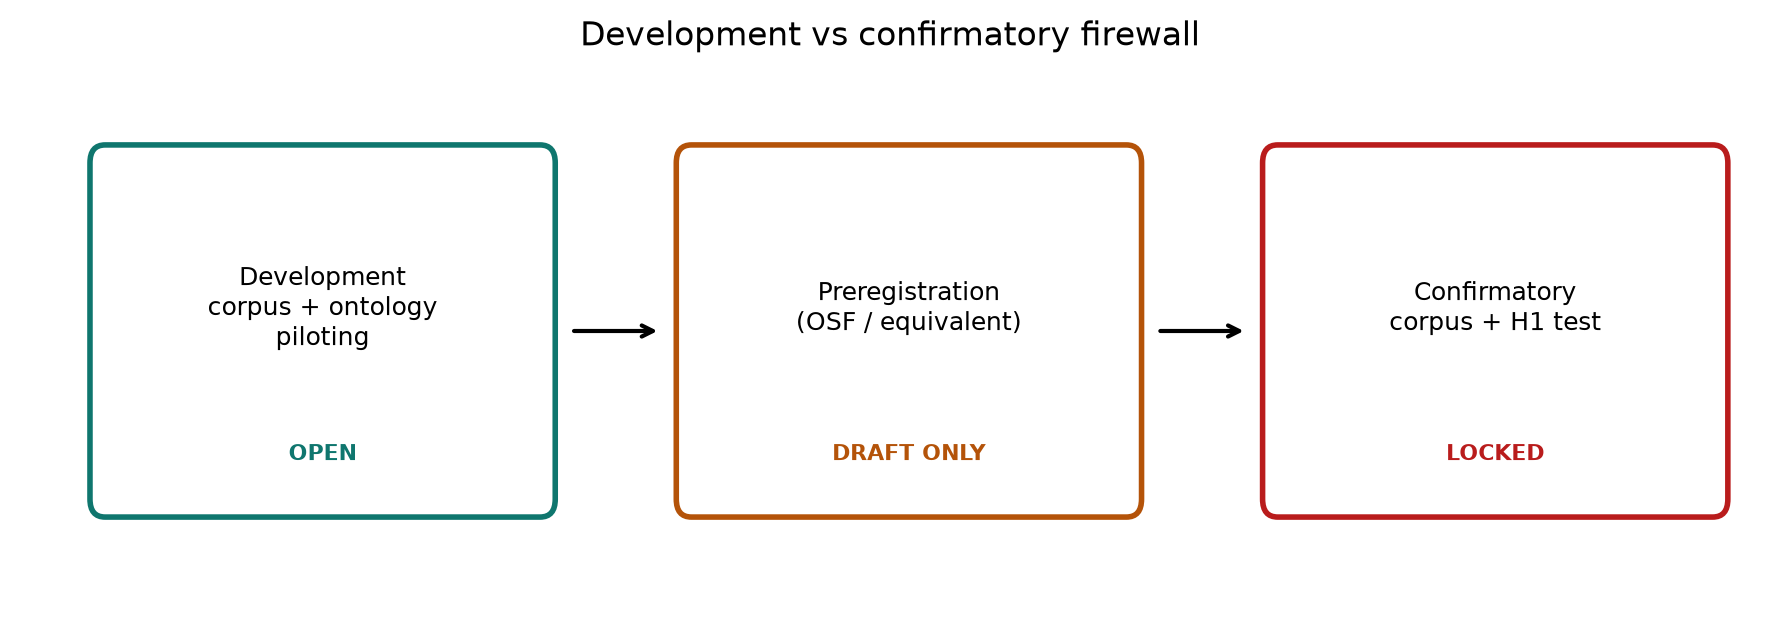
\includegraphics[width=0.95\linewidth]{figures/fig04_firewall.png}
\caption{Development vs confirmatory firewall; confirmatory analysis remains locked.}
\label{fig:firewall}
\end{figure}
% Auto-generated — do not edit by hand
% Generated: 2026-08-15T18:05:51.965429+00:00
\begin{table}[t]
\centering
\caption{Project status gates (honest incomplete items listed).}
\label{tab:status}
\begin{tabular}{ll}
\toprule
gate & status \\
\midrule
Ontology v0.1 & PILOTED \\
Synthetic E2E pipeline & COMPLETE \\
Positive-control instrument tests & PASSING \\
Human validation & REQUIRES\_EXTERNAL\_HUMAN\_VALIDATION \\
OSF preregistration & READY\_FOR\_EXTERNAL\_PREREGISTRATION \\
Confirmatory analysis & LOCKED \\
Licensed development corpus (500-800) & IN\_PROGRESS\_POINTERS \\
Expert Sanskrit review & REQUIRES\_EXPERT\_REVIEW \\
Expert physicist review & REQUIRES\_EXPERT\_REVIEW \\
\bottomrule
\end{tabular}
\end{table}

Licensing: copyrighted scholarly translations are bibliographic pointers unless redistribution is permitted (\texttt{docs/DATA\_STATEMENT.md}).

\section{Ontology and Annotation}
Ontology v0.1 encodes 36 physics-derived structural features.
\begin{figure}[H]
\centering
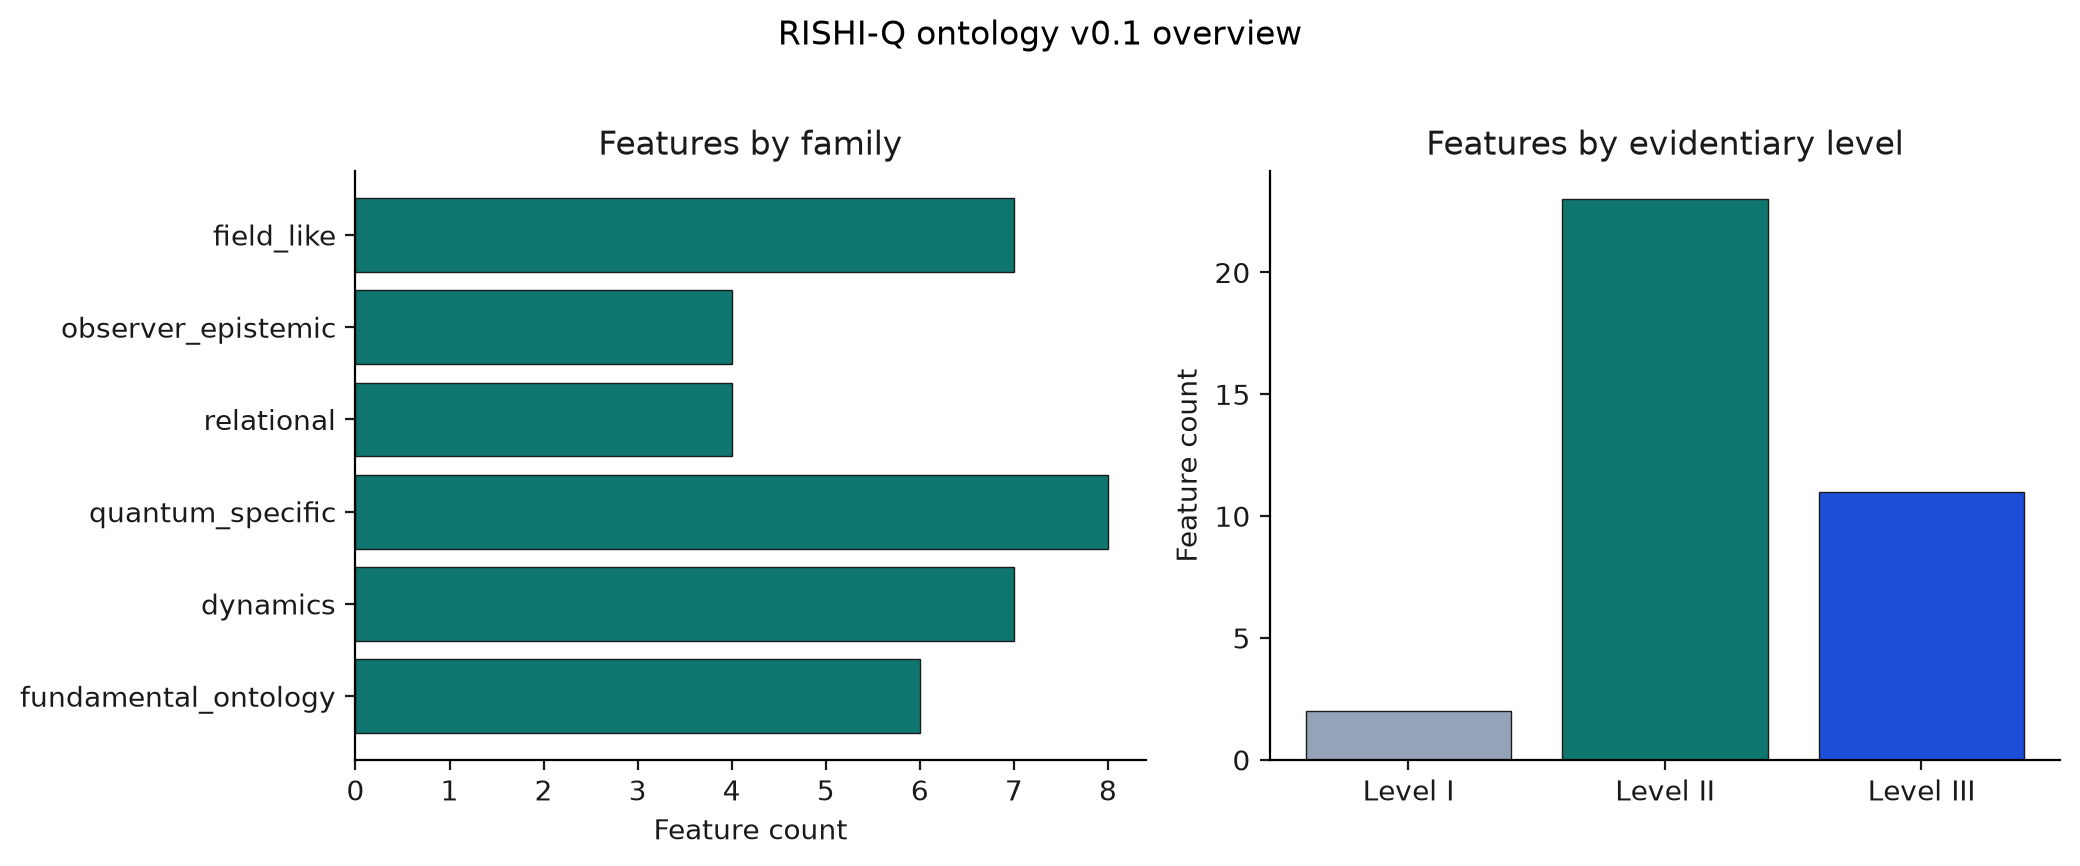
\includegraphics[width=\linewidth]{figures/fig03_ontology_overview.png}
\caption{Ontology inventory by family and evidentiary level.}
\label{fig:ontology}
\end{figure}
\begin{figure}[H]
\centering
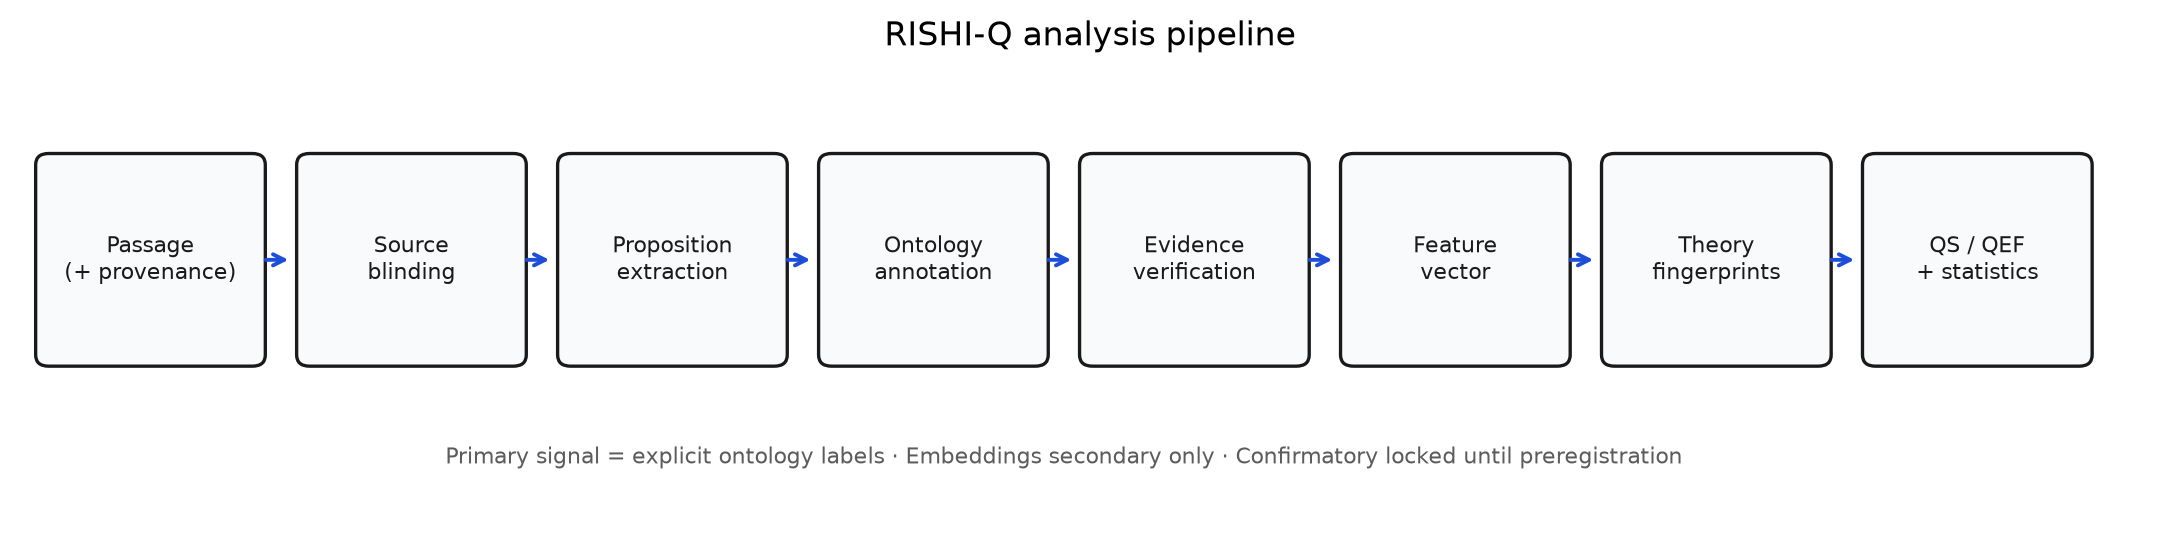
\includegraphics[width=\linewidth]{figures/fig01_pipeline.png}
\caption{System~A analysis pipeline. Embeddings are secondary only.}
\label{fig:pipeline}
\end{figure}
Positive labels require exact evidence spans.
Local development uses a deterministic heuristic backend; Kaggle notebooks support open-model replication.

\section{System~B: Computational Discovery Engine}
\subsection{Concept graphs}
Passages are represented not only as feature vectors but as evidence-bound concept graphs (nodes such as substrate, state, observer; edges such as \texttt{pervades}, \texttt{manifests\_as}).
Edges are never invented without positive labels and evidence spans.
\begin{figure}[H]
\centering
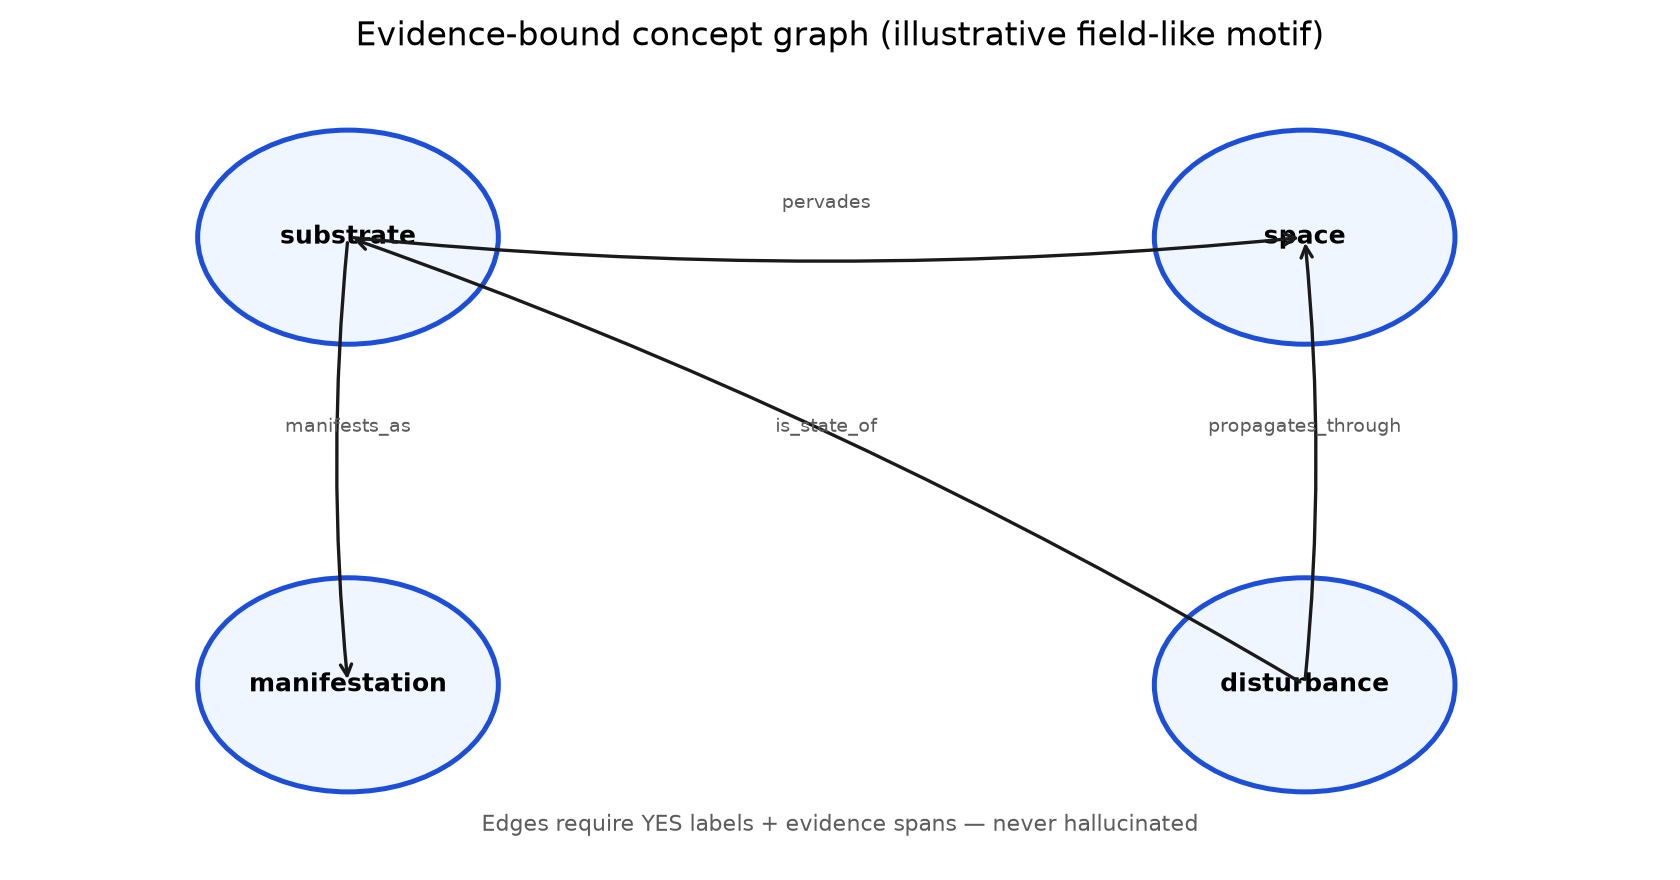
\includegraphics[width=0.92\linewidth]{figures/fig25_concept_graph.png}
\caption{Illustrative evidence-bound concept graph (field-like motif shape).}
\label{fig:graph}
\end{figure}

\subsection{Label-free motif discovery}
\begin{figure}[H]
\centering
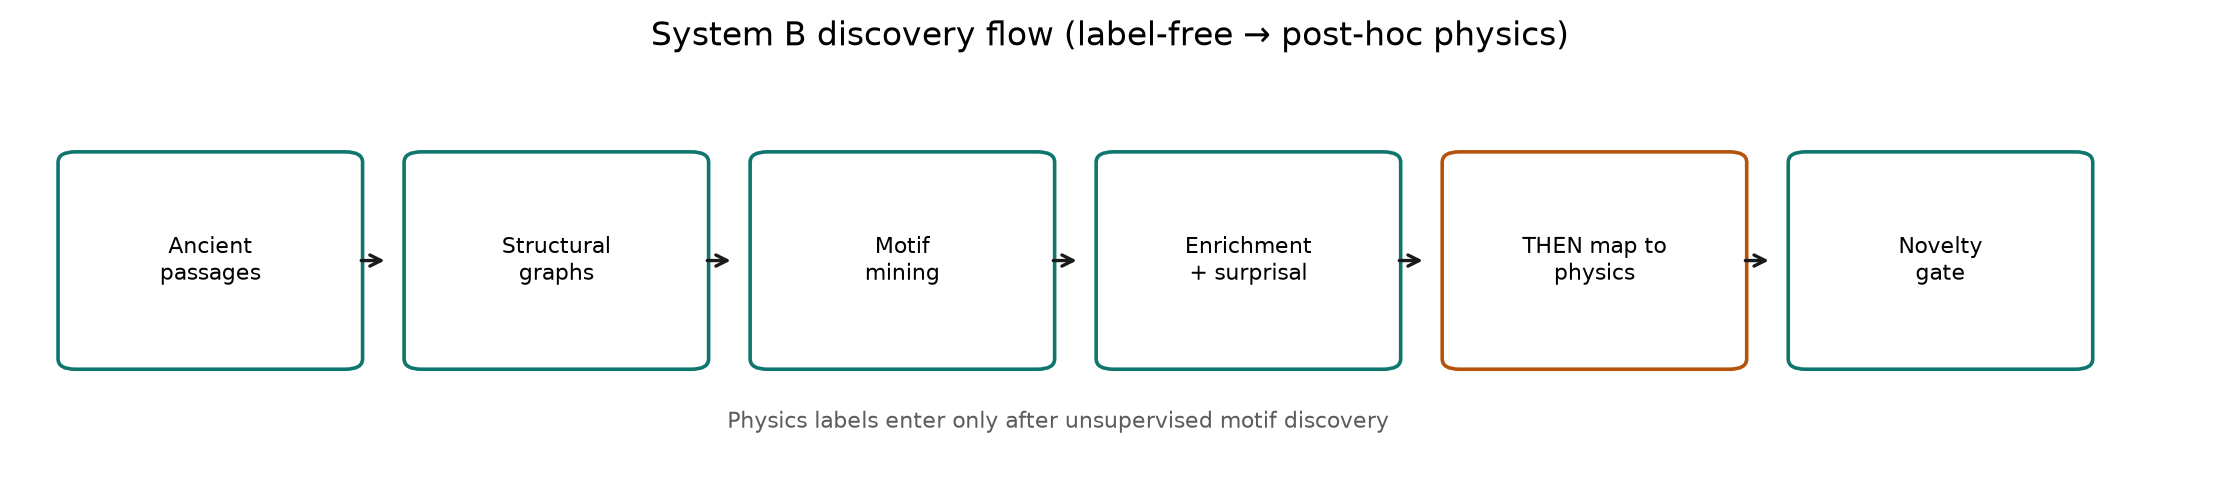
\includegraphics[width=\linewidth]{figures/fig24_discovery_flow.png}
\caption{Discovery flow: physics labels enter only after unsupervised motif mining.}
\label{fig:discflow}
\end{figure}
Recurring structural signatures are mined as \emph{Rishi Motifs}.
Only afterward are motifs compared to Newtonian, classical-field, thermodynamic, relativistic, QM, and QFT fingerprints.

\subsection{Significance without p-hacking}
Motif enrichment uses tradition contrasts and work-cluster bootstrap.
Ranking combines effect size, replication across works, specificity, and robustness---not $p$-value primacy.
Discovery/replication splits are work-stratified to reduce leakage.
Exploratory candidates remain exploratory until frozen and tested on held-out works.

\section{Statistics}
Inference respects passage $\subset$ section $\subset$ work $\subset$ tradition.
Planned tools: mixed-effects models, cluster bootstrap CIs, cluster-preserving permutation tests, BH--FDR for secondary tests, and power simulation.
\begin{figure}[H]
\centering
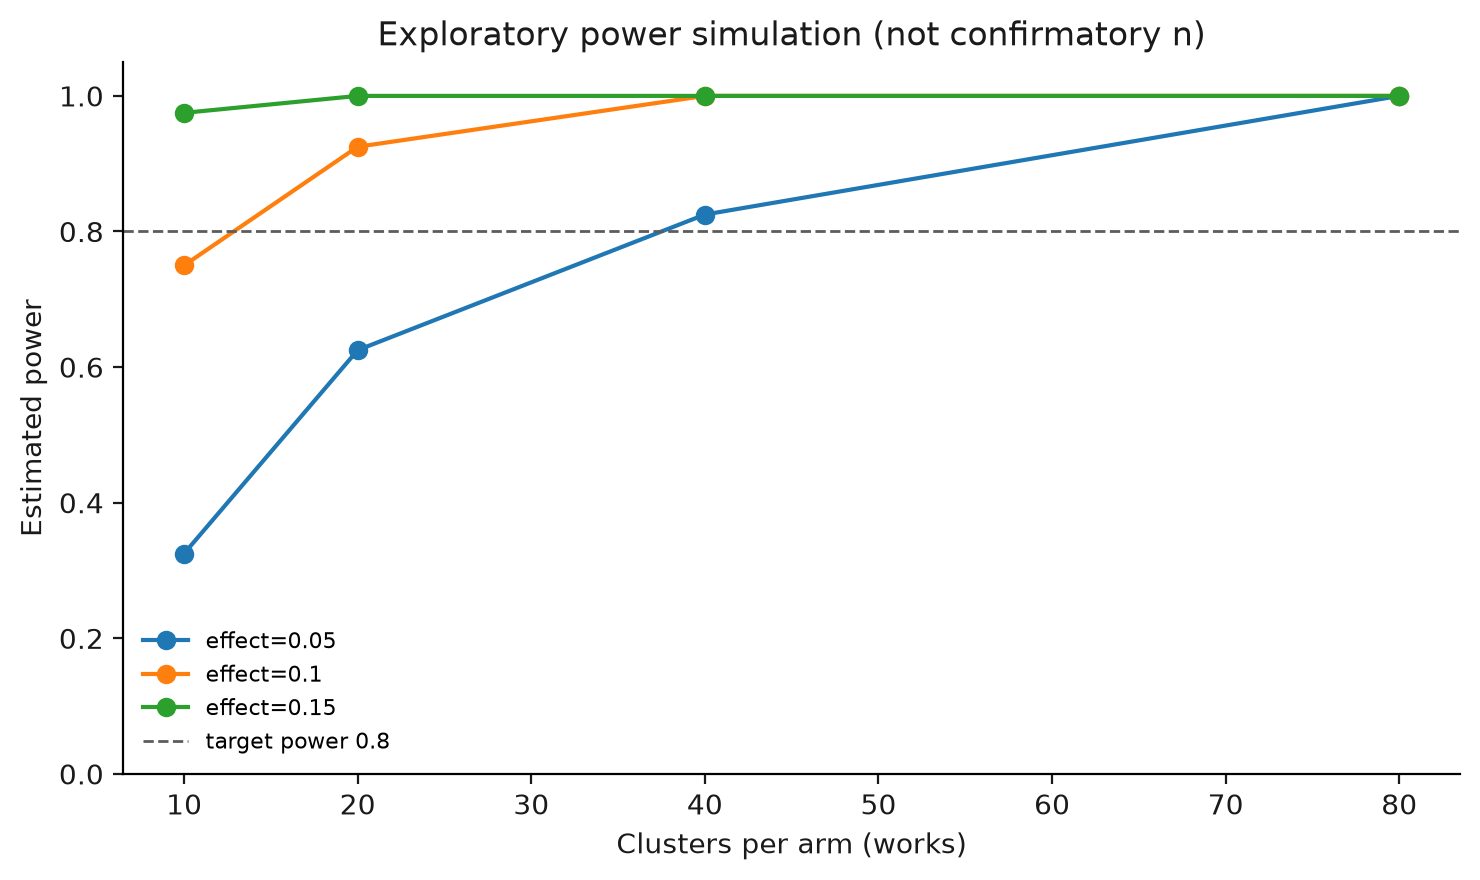
\includegraphics[width=0.85\linewidth]{figures/fig11_power_curves.png}
\caption{Exploratory power curves. Confirmatory $n$ not frozen.}
\label{fig:power}
\end{figure}

\section{Instrument Validation (Synthetic Controls)}
\label{sec:instrument}
These results validate the measurement instrument, not H1.
\begin{figure}[H]
\centering
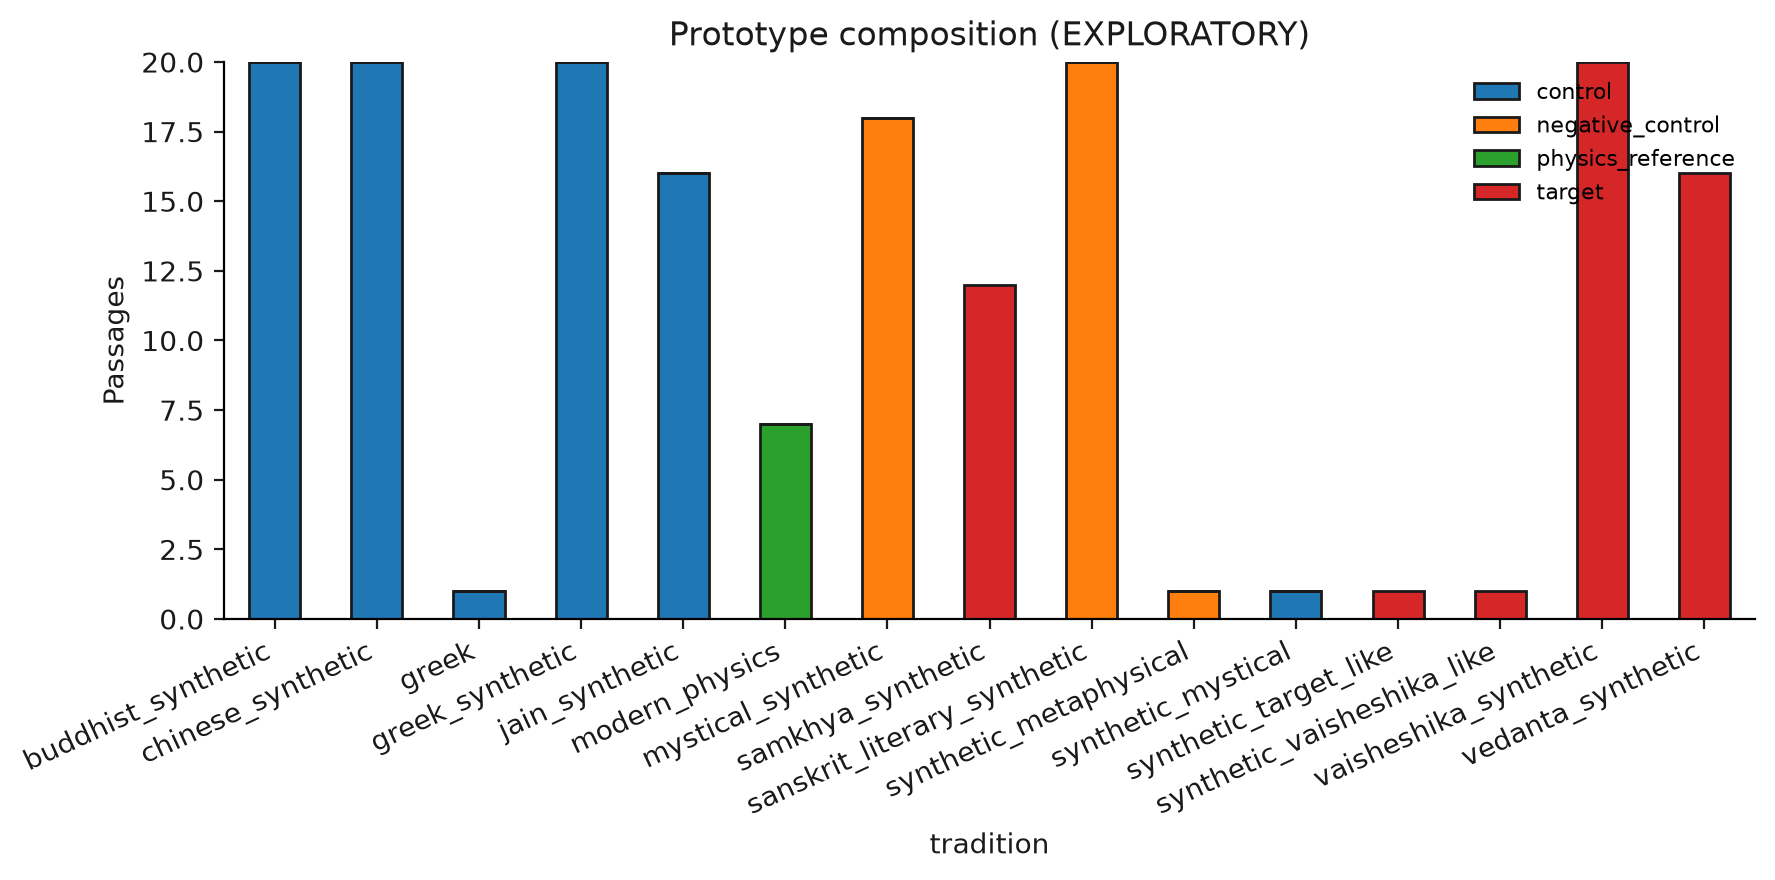
\includegraphics[width=\linewidth]{figures/fig17_prototype_balance.png}
\caption{Development prototype composition (protocol §95-style panel; synthetic).}
\label{fig:balance}
\end{figure}
\begin{figure}[H]
\centering
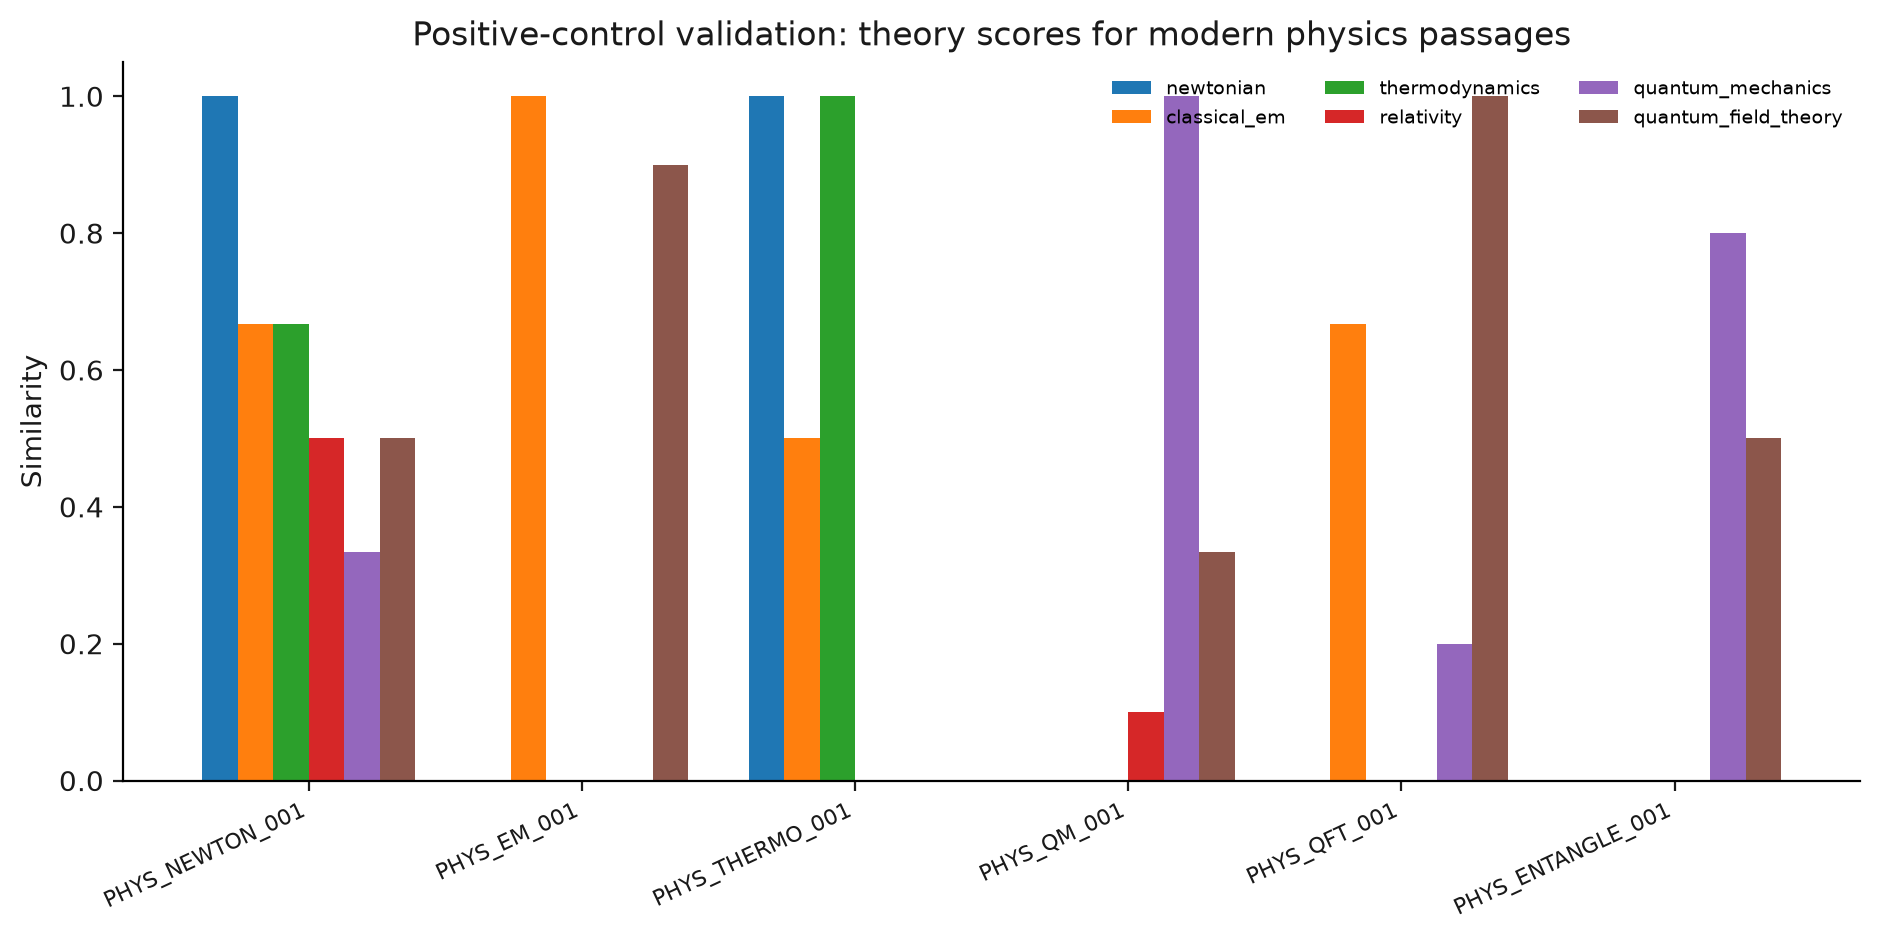
\includegraphics[width=\linewidth]{figures/fig05_positive_controls.png}
\caption{Theory similarities for modern-physics control passages.}
\label{fig:poscontrols}
\end{figure}
% Auto-generated — do not edit by hand
% Generated: 2026-08-15T18:05:51.920622+00:00
\begin{table}[t]
\centering
\caption{Positive-control instrument check on modern physics passages.}
\label{tab:positive-controls}
\begin{tabular}{lllllll}
\toprule
passage\_id & work & QS & QEF & quantum\_mechanics & classical\_em & expected\_emphasis \\
\midrule
PHYS\_NEWTON\_001 & Synthetic Newtonian description & -0.500 & 0.000 & 0.333 & 0.667 & classical mechanics \\
PHYS\_EM\_001 & Synthetic classical EM description & -0.100 & 0.000 & 0.000 & 1.000 & classical EM / field \\
PHYS\_THERMO\_001 & Synthetic thermodynamics description & -1.000 & 0.000 & 0.000 & 0.500 & thermo / epistemic \\
PHYS\_QM\_001 & Synthetic QM description & 0.900 & 1.000 & 1.000 & 0.000 & quantum mechanics \\
PHYS\_QFT\_001 & Synthetic QFT description & 0.333 & 1.000 & 0.200 & 0.667 & QFT \\
PHYS\_ENTANGLE\_001 & Synthetic entanglement description & 0.800 & 1.000 & 0.800 & 0.000 & nonseparability \\
\bottomrule
\end{tabular}
\end{table}

Unity metaphors do not trigger nonseparability; QM/QFT controls yield high $QS$/$QEF$ as required.
\begin{figure}[H]
\centering
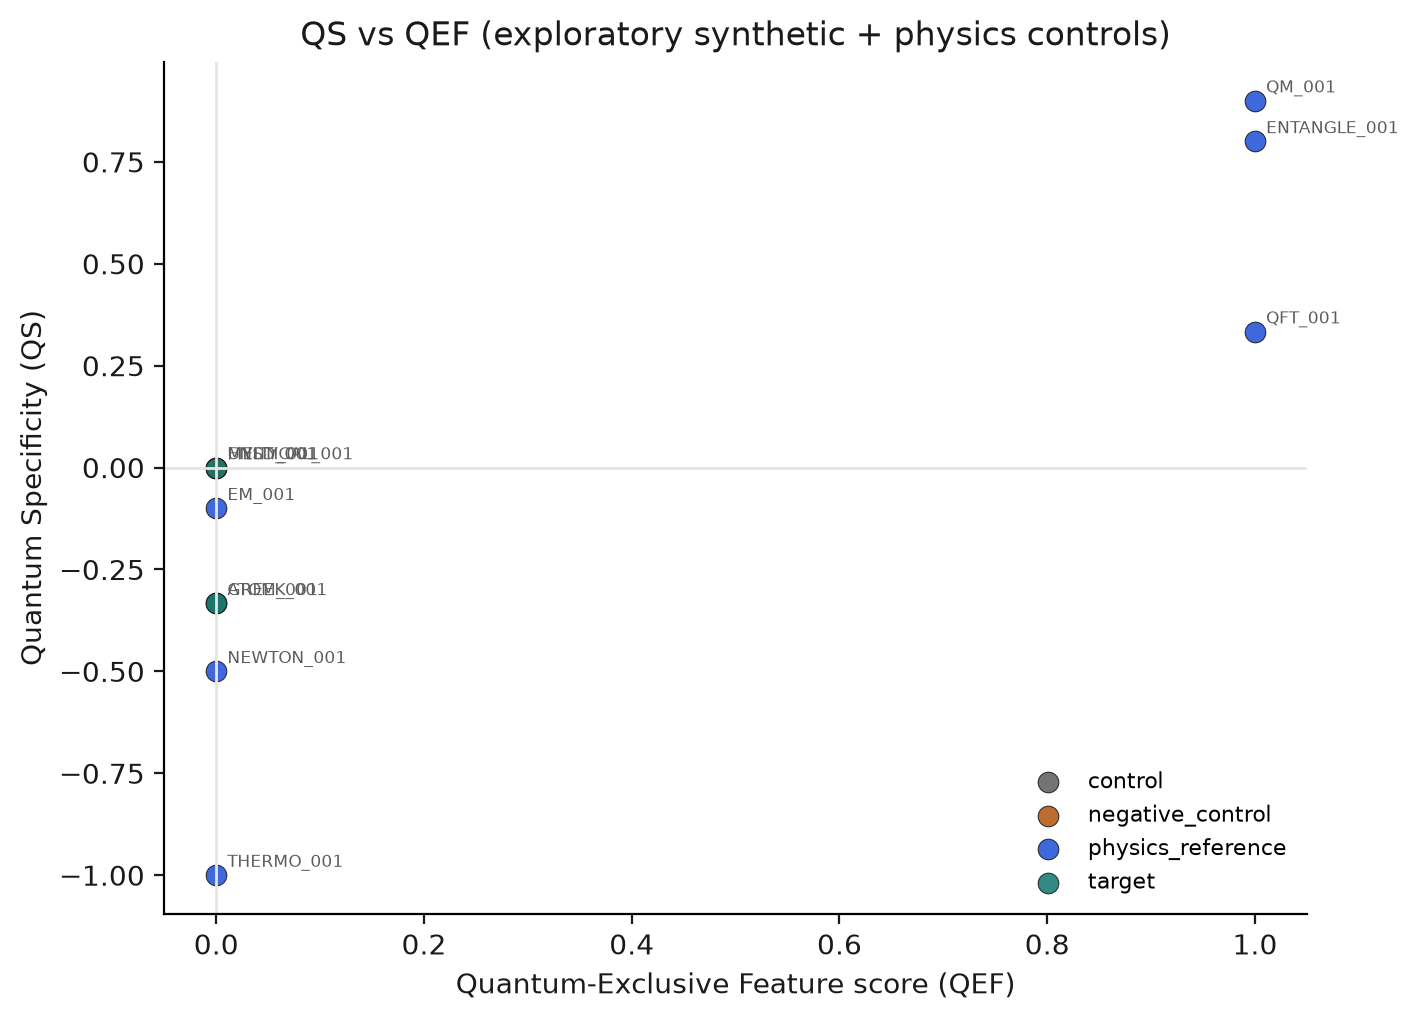
\includegraphics[width=0.82\linewidth]{figures/fig08_qs_qef_scatter.png}
\caption{$QS$ vs $QEF$ on seed physics/control passages.}
\label{fig:scatter}
\end{figure}
On prototype100, target-like synthetic slices are near-null relative to controls ($\Delta_Q\approx -0.015$, $p\approx 0.58$).
\begin{figure}[H]
\centering
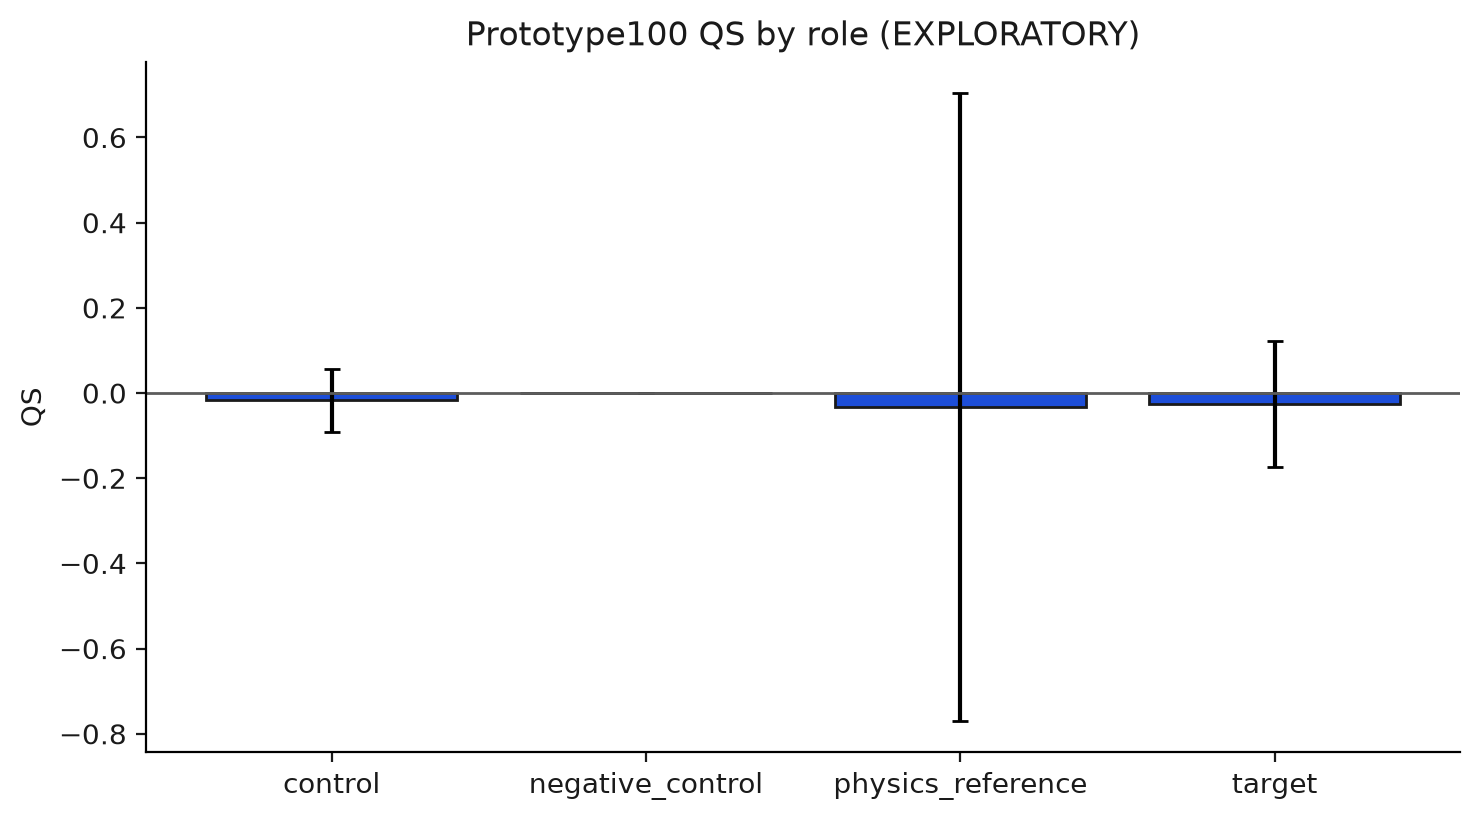
\includegraphics[width=0.85\linewidth]{figures/fig14_prototype100_qs_by_role.png}
\caption{QS by role on prototype100 (exploratory).}
\label{fig:qsrole}
\end{figure}
\begin{figure}[H]
\centering
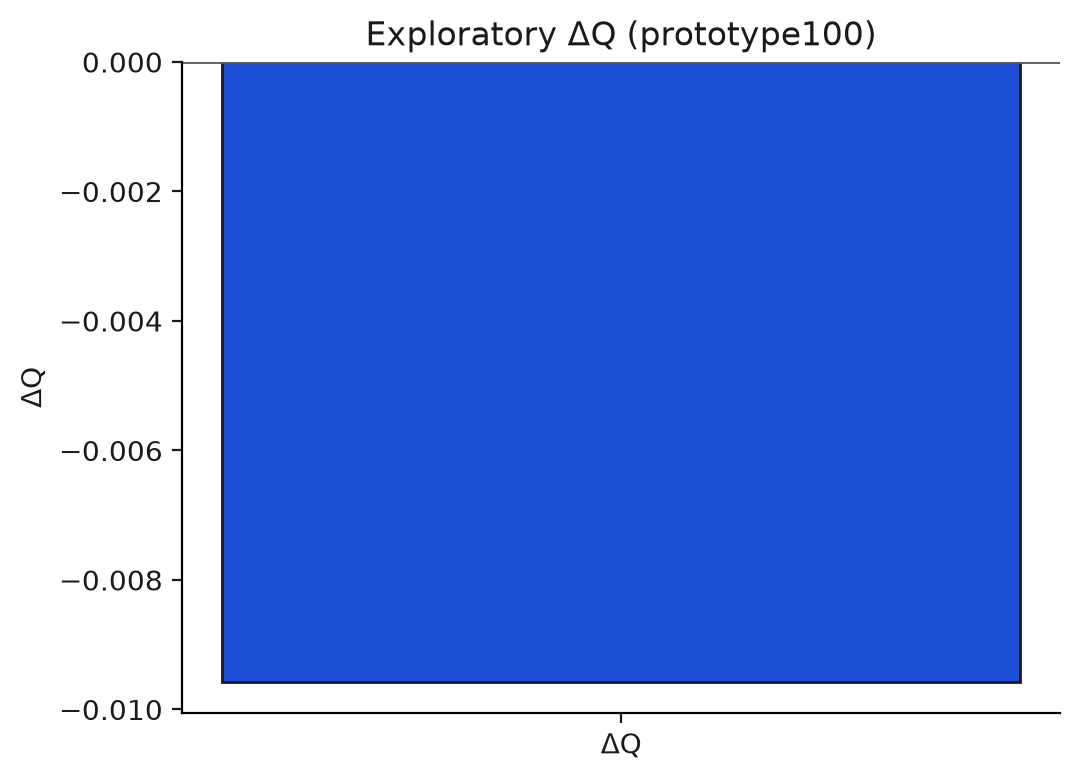
\includegraphics[width=0.8\linewidth]{figures/fig16_primary_effect_exploratory.png}
\caption{Exploratory $\Delta_Q$ (not confirmatory).}
\label{fig:delta}
\end{figure}
\begin{figure}[H]
\centering
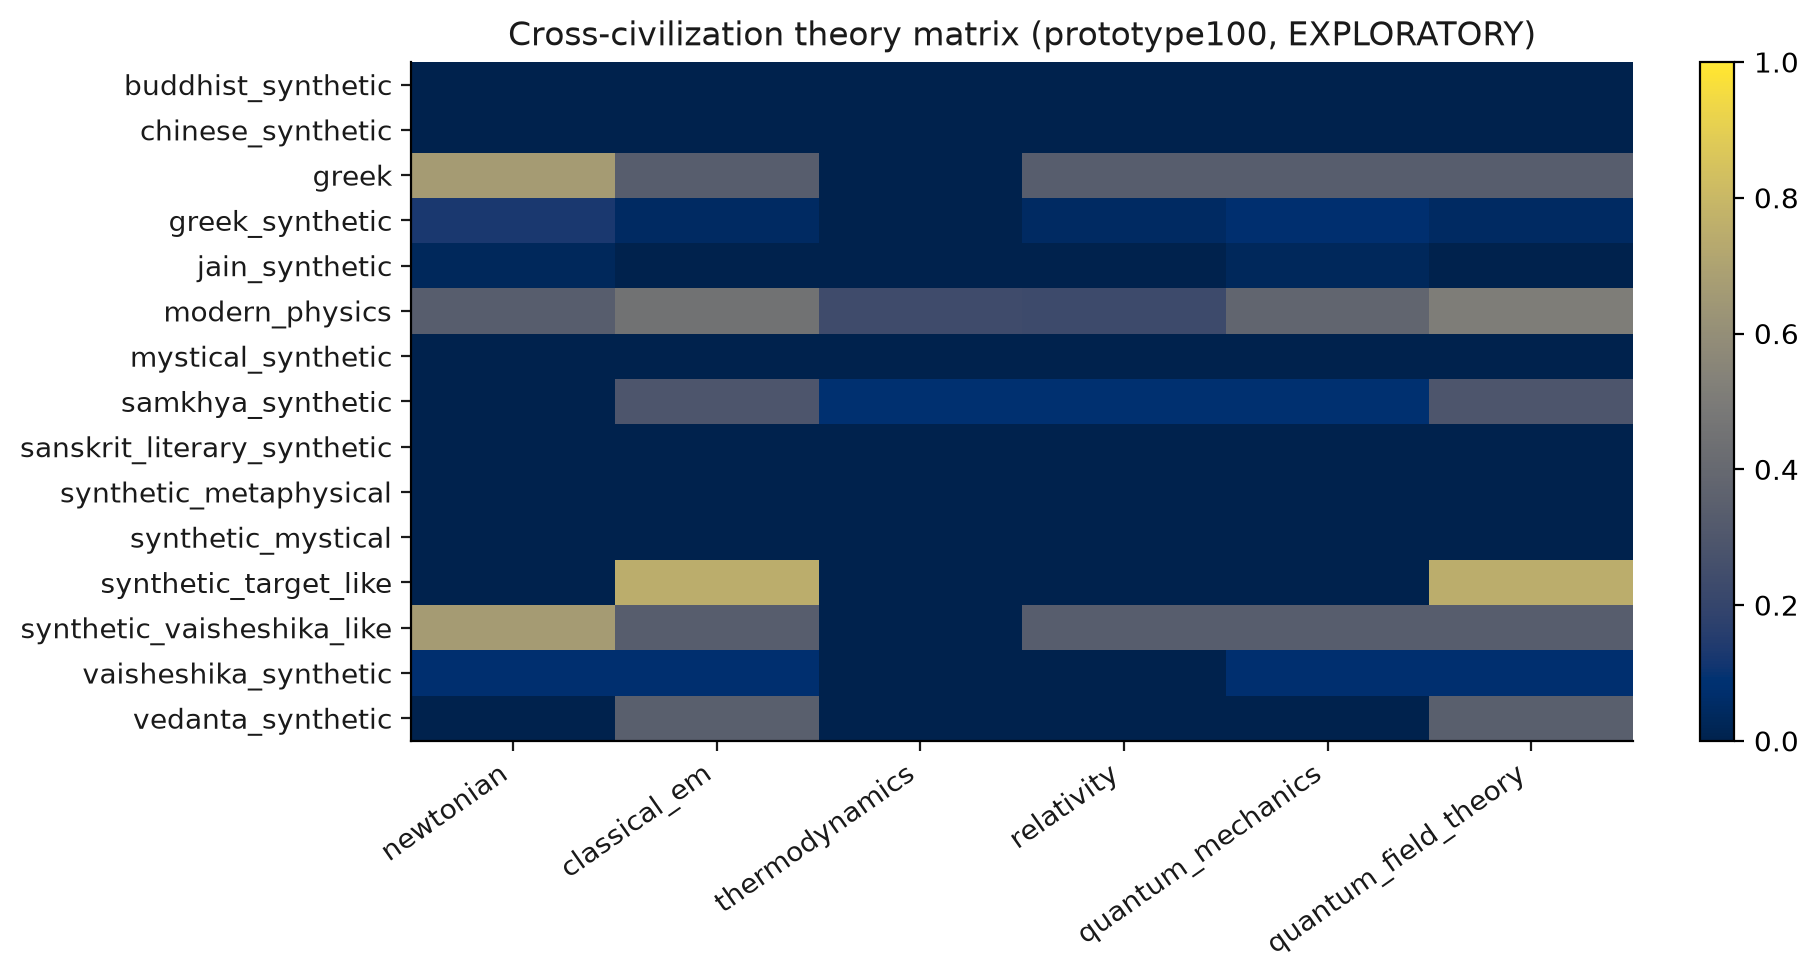
\includegraphics[width=\linewidth]{figures/fig13_cross_civilization.png}
\caption{Cross-civilization theory tournament (exploratory synthetic panel).}
\label{fig:tournament}
\end{figure}
\begin{figure}[H]
\centering
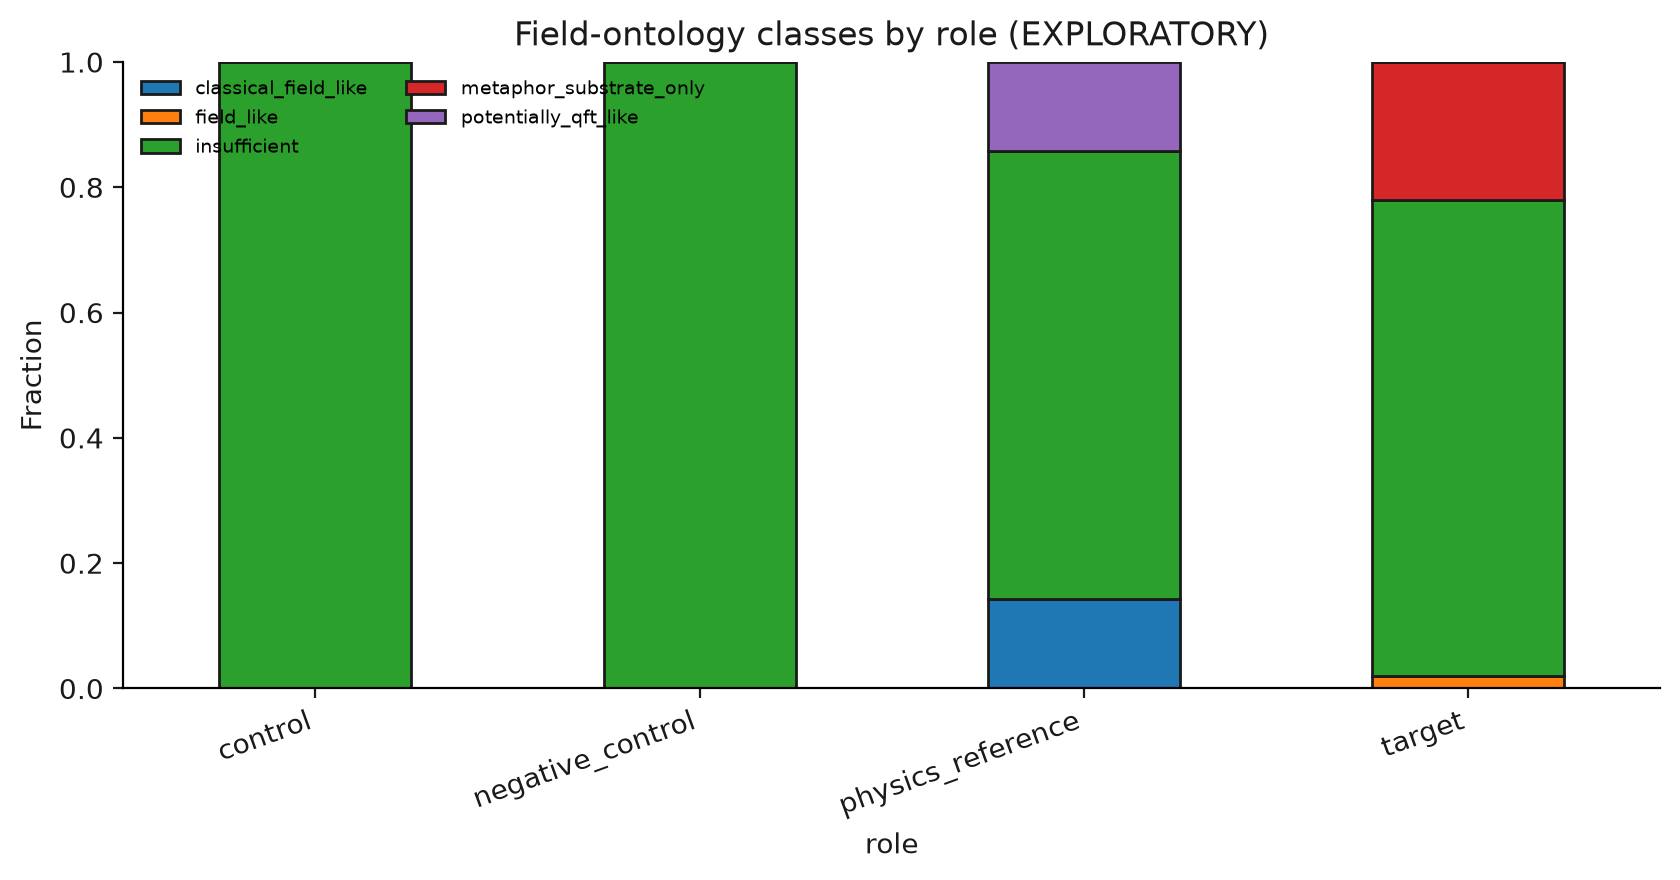
\includegraphics[width=\linewidth]{figures/fig15_field_ontology.png}
\caption{Field-ontology class fractions by role.}
\label{fig:field}
\end{figure}

\section{Exploratory Public-Domain Pilot}
A public-domain English development panel ($n=276$: Upani\d{s}ads/Paramananda; Lucretius; Timaeus; Dhammapada; \emph{Tao Te Ching}; plus physics controls) was annotated with the heuristic backend.
Under this annotator, historical slices sit near the annotation floor ($\Delta_Q\approx 0$, $\mathrm{QEF}=0$), while physics controls still discriminate---an \emph{instrument limitation} finding, not a confirmatory Sanskrit null.
\begin{figure}[H]
\centering
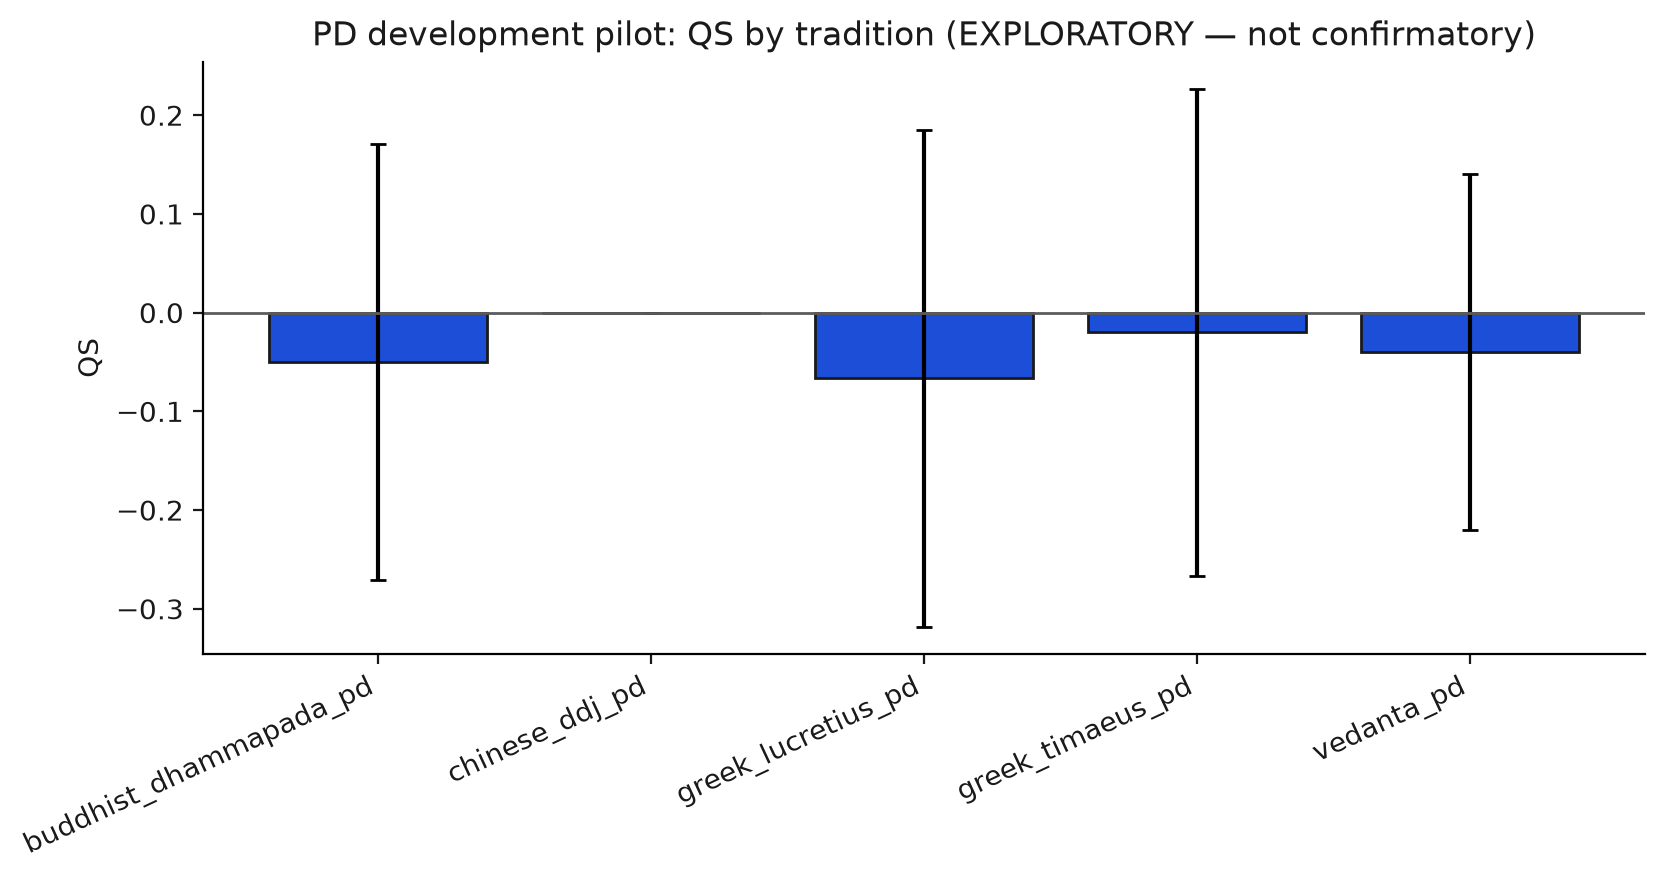
\includegraphics[width=\linewidth]{figures/fig18_pd_pilot_qs.png}
\caption{PD pilot QS by tradition (EXPLORATORY).}
\label{fig:pdqs}
\end{figure}
\begin{figure}[H]
\centering
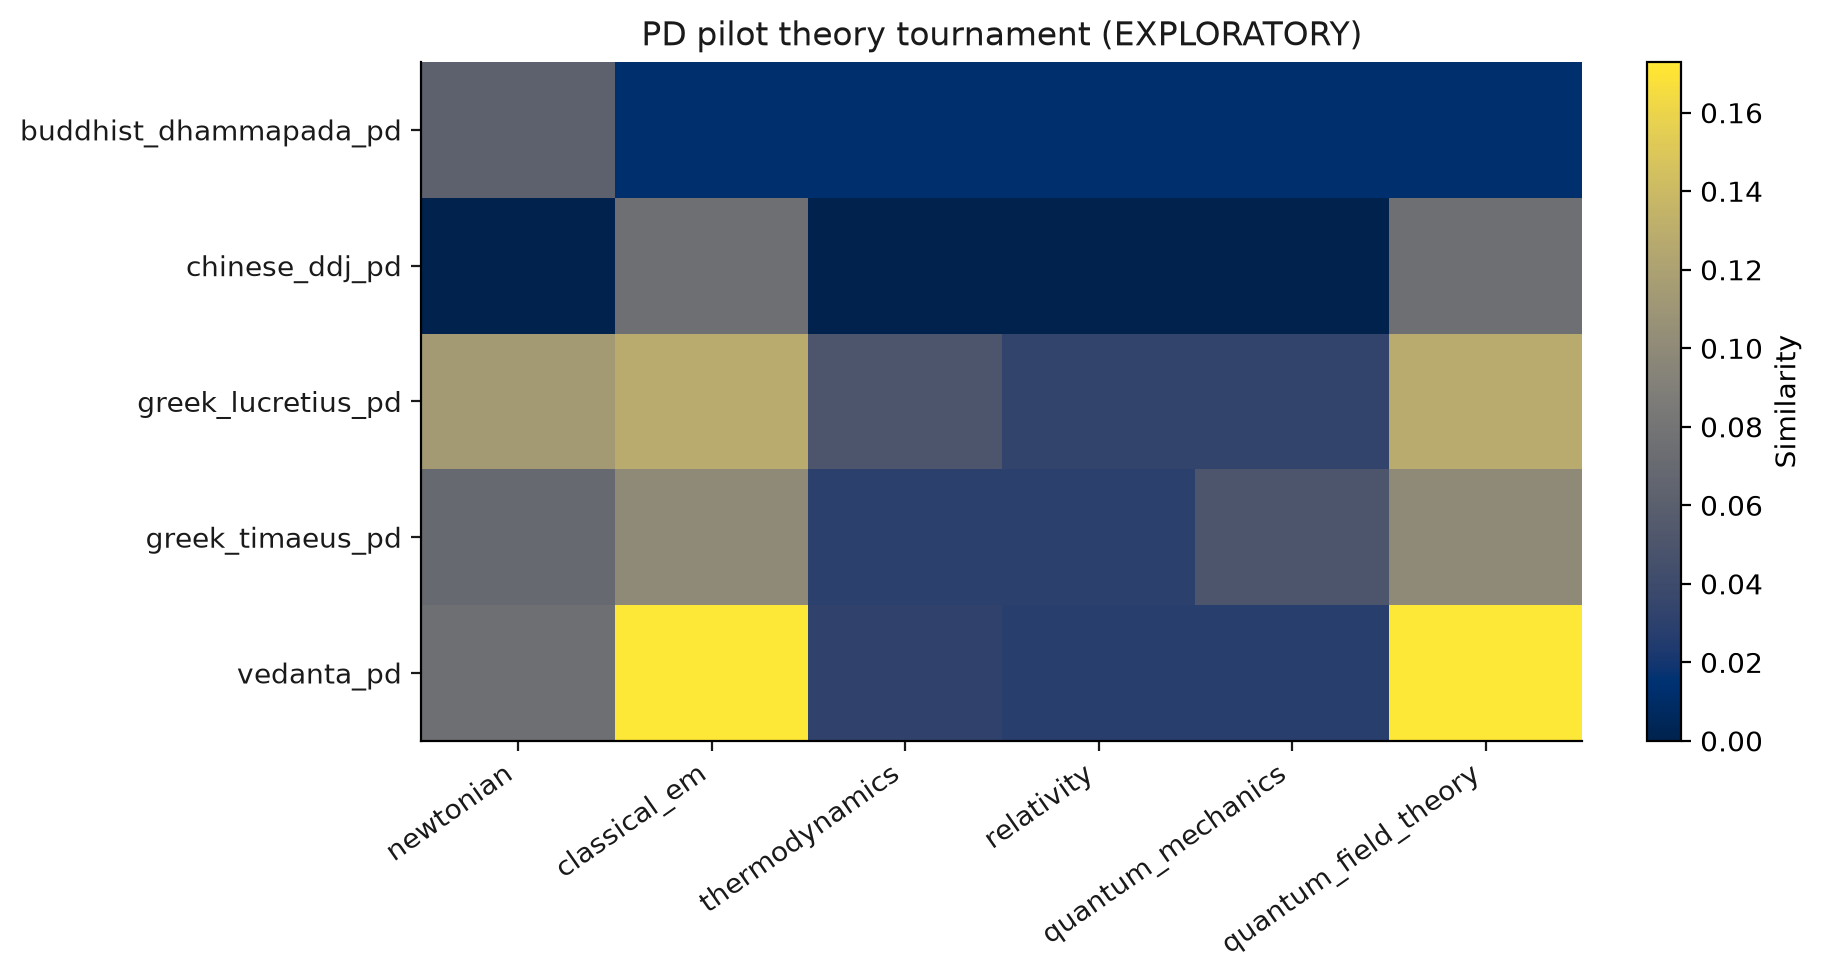
\includegraphics[width=\linewidth]{figures/fig19_pd_pilot_tournament.png}
\caption{PD pilot theory tournament (EXPLORATORY).}
\label{fig:pdtourn}
\end{figure}
Settlement of H1 requires LLM/human annotation and preregistration.

\section{Flagship finding: Capra-style claim autopsy}
\label{sec:flagship}
Popular culture asserts that Sanskrit wisdom anticipated quantum physics.
On the public-domain Ved\={a}nta panel, a curated autopsy of Capra-style claims finds the reverse pattern:

\begin{quote}
\textbf{Five of five} curated Capra-style claims are classified \texttt{CONTRADICTED\_AS\_QUANTUM}:
Level~I/II metaphysical components appear in the sample, while quantum-specific (Level~III) components do not.
Masking modern physics lexicon does not manufacture quantum signal (mean $\Delta QS\approx +0.006$ on Ved\={a}nta).
The PD ``electrons'' sentence is Paramananda's 1919 commentary \emph{rejecting} material science as a path to Brahman---the rhetorical opposite of Capra-style co-option.
\end{quote}

\begin{figure}[H]
\centering
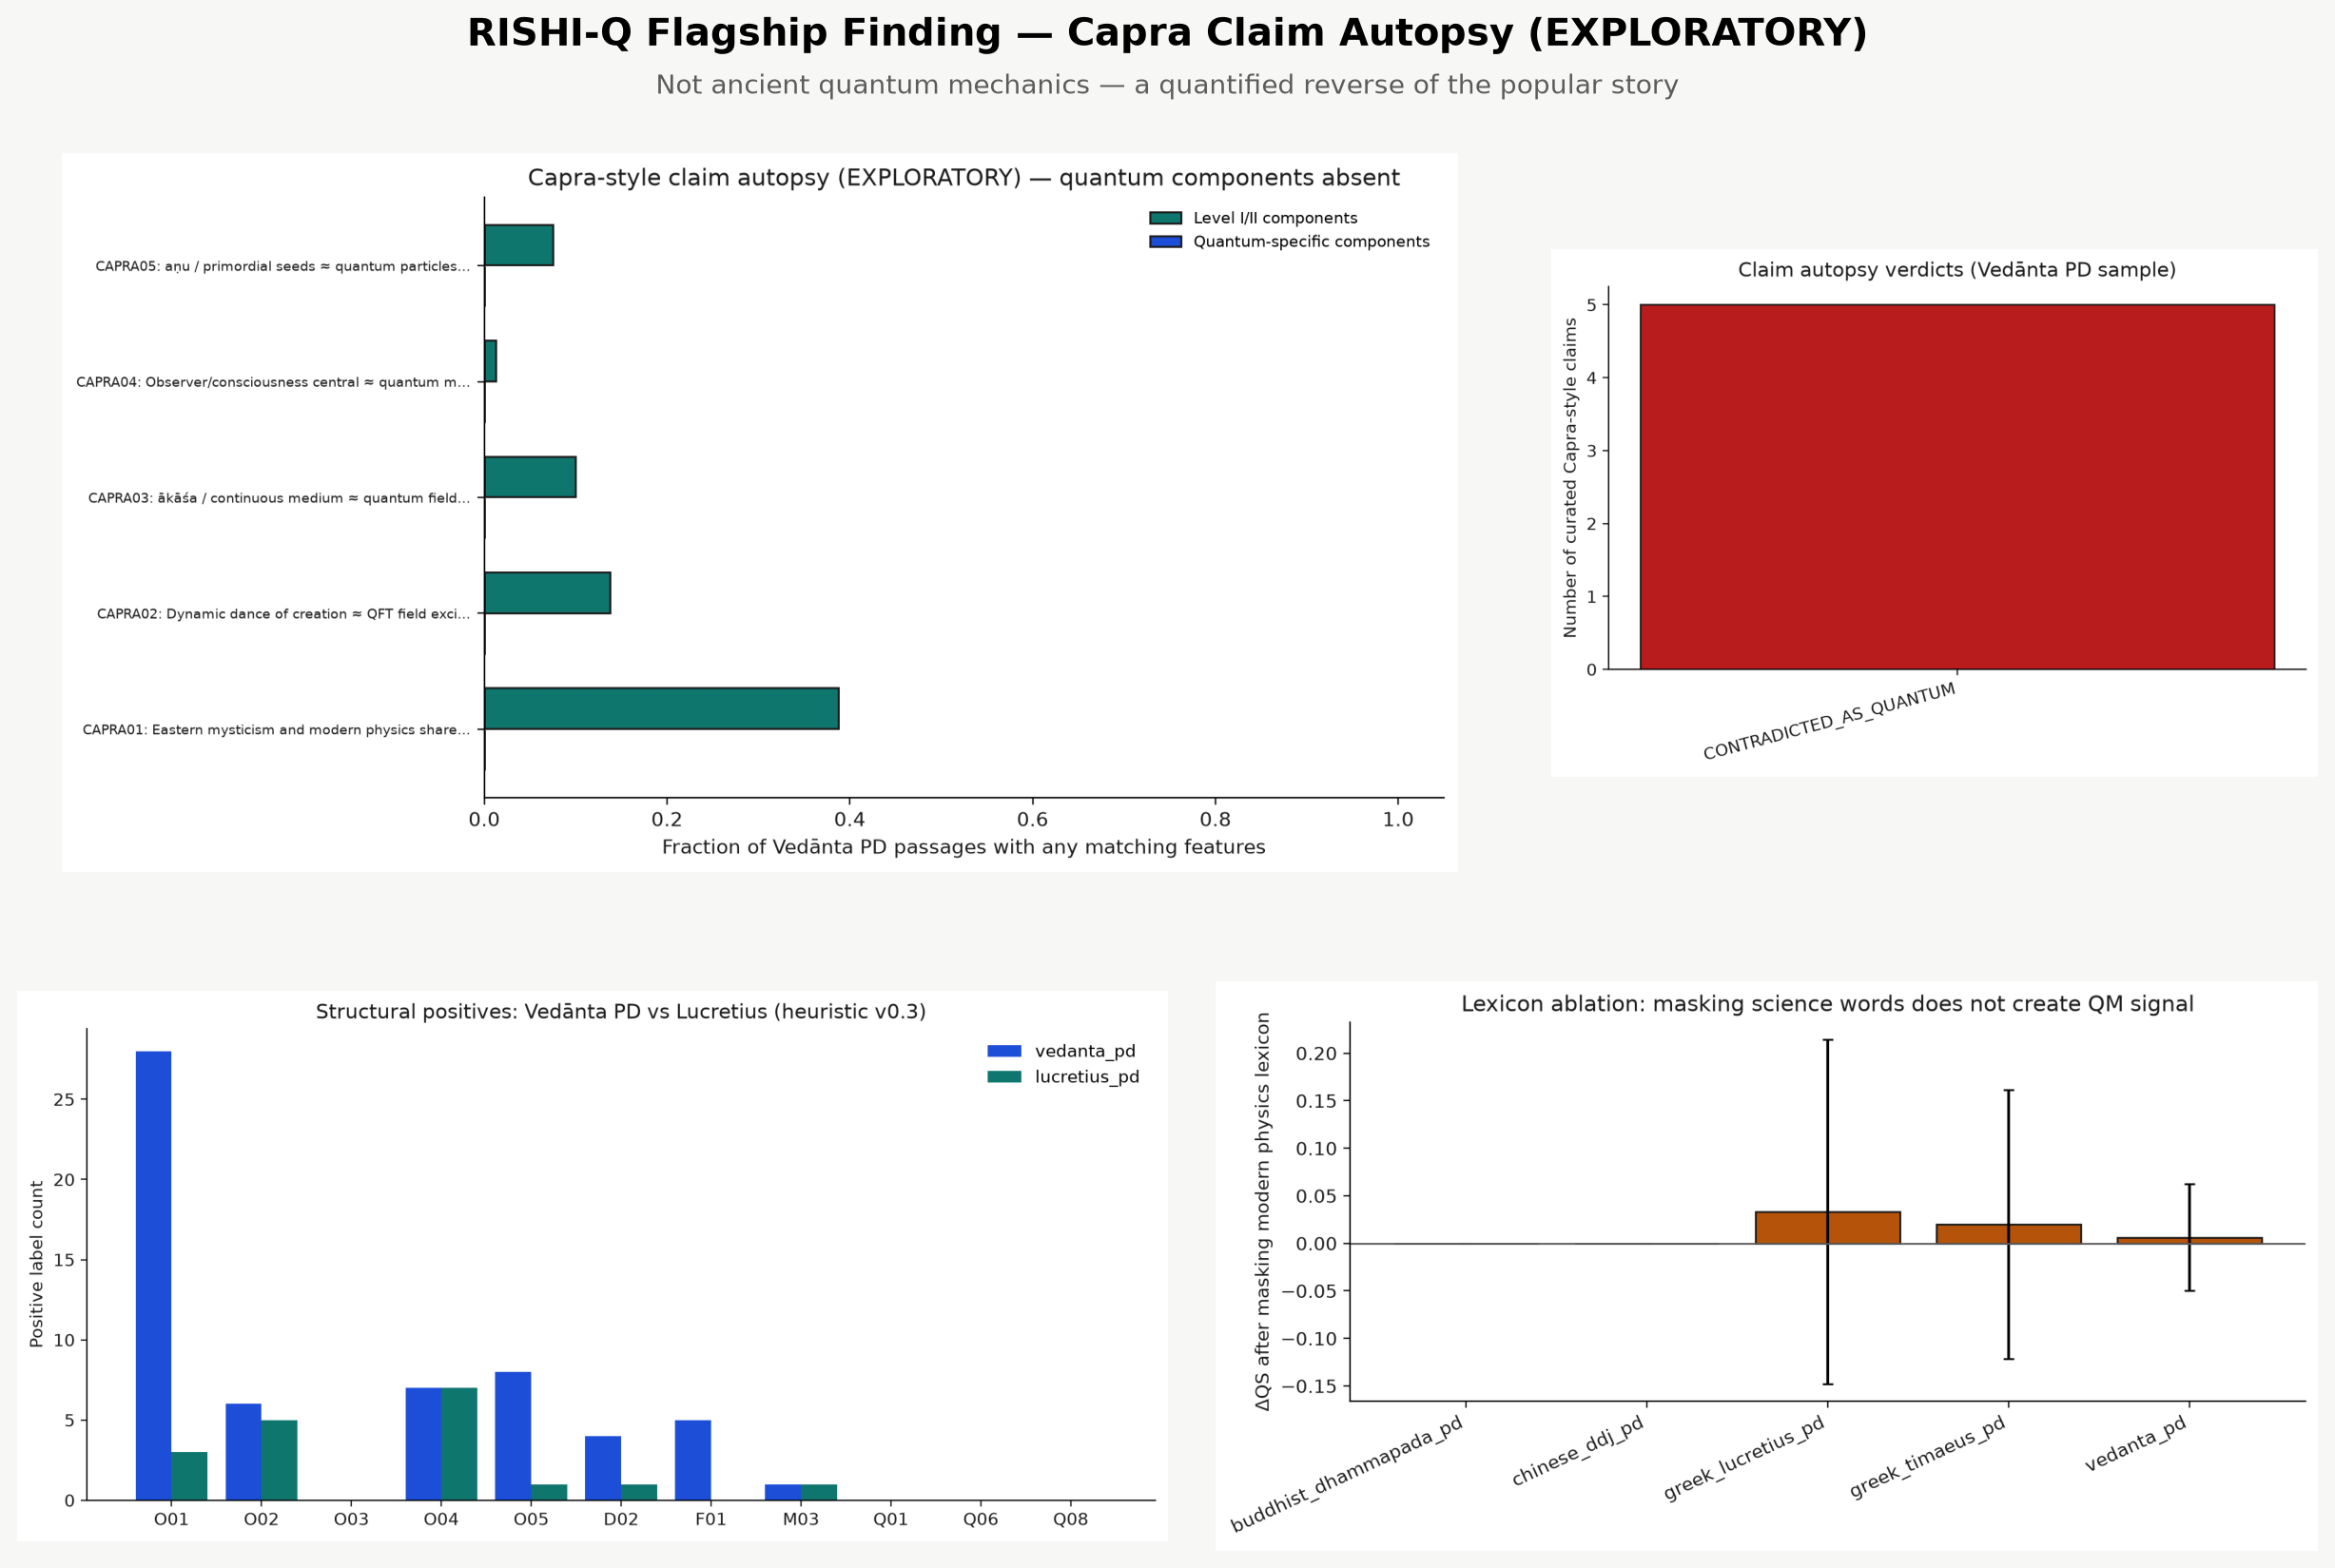
\includegraphics[width=\linewidth]{figures/fig38_flagship_poster.png}
\caption{Flagship exploratory poster: Capra autopsy, tradition contrast, lexicon ablation.}
\label{fig:flagship}
\end{figure}
\begin{figure}[H]
\centering
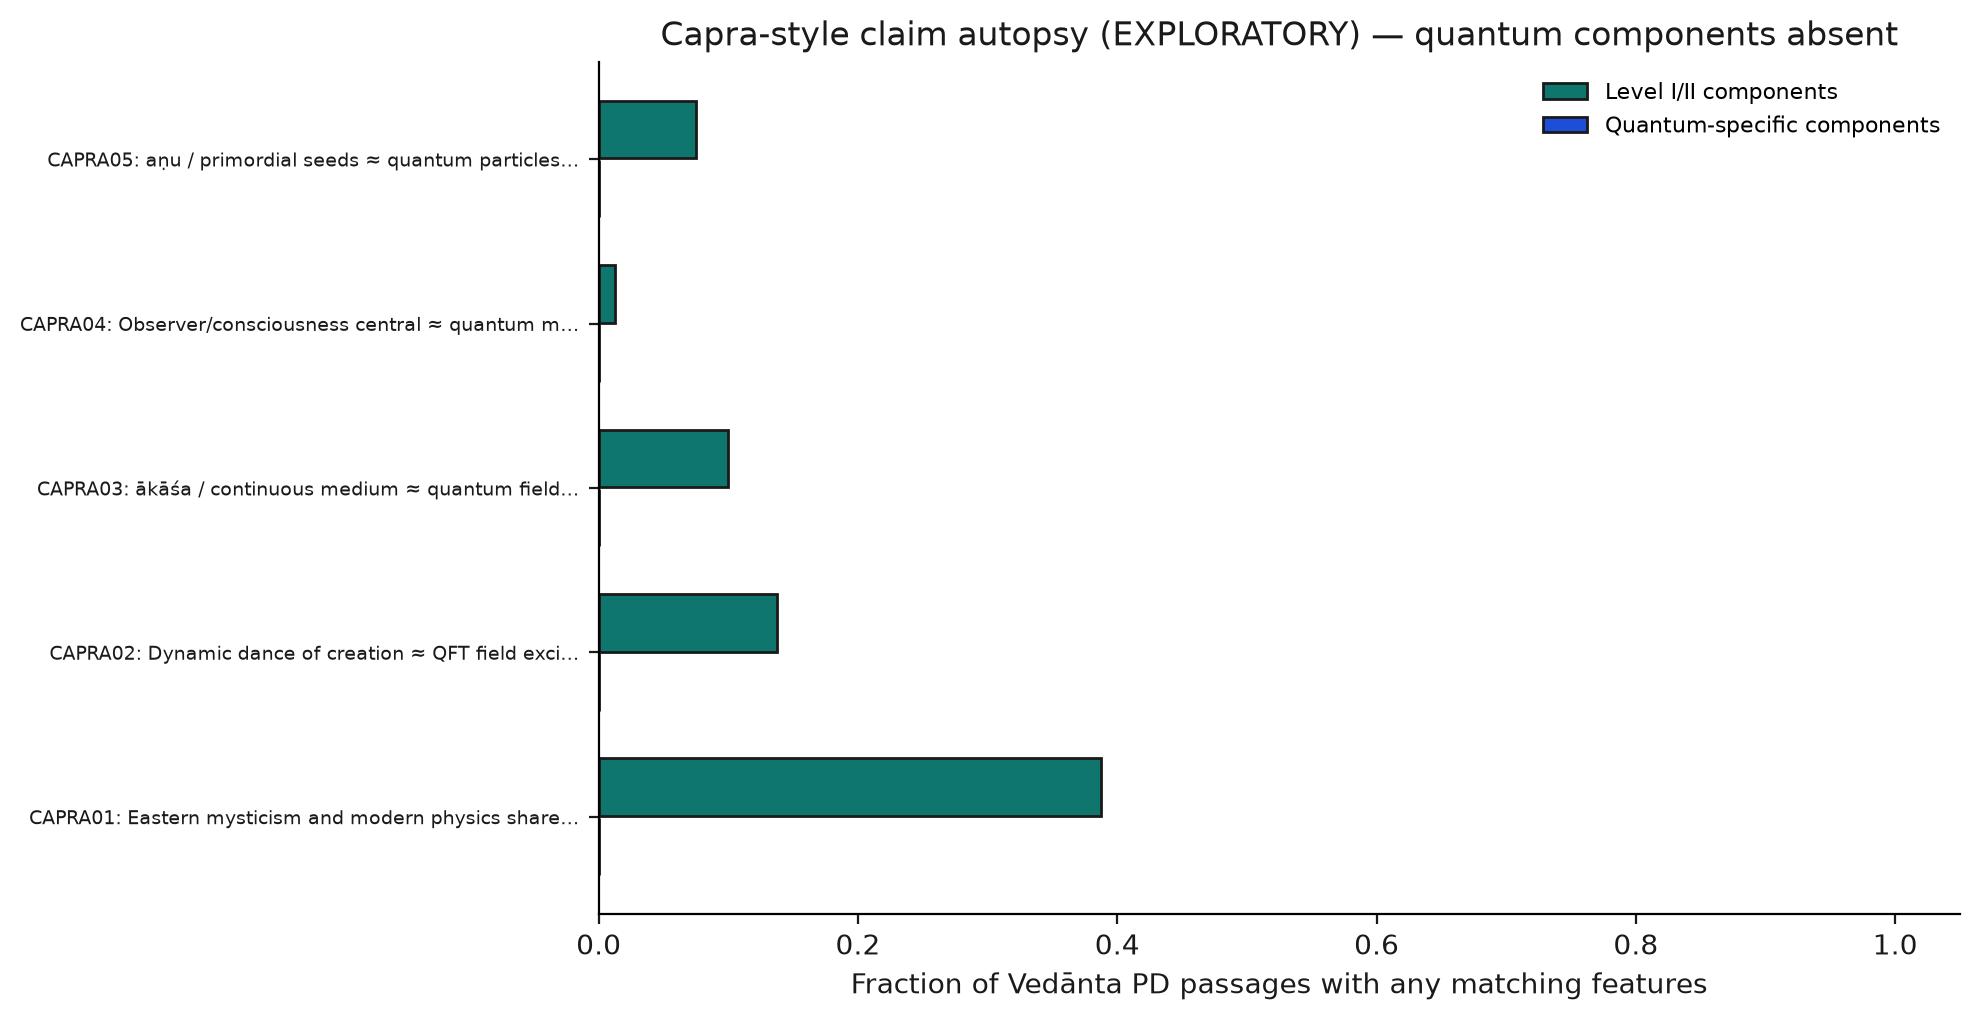
\includegraphics[width=\linewidth]{figures/fig35_capra_claim_autopsy.png}
\caption{Capra-style claim autopsy on Ved\={a}nta PD (EXPLORATORY).}
\label{fig:capra}
\end{figure}
This is a Tier~2--3 quantitative finding about how quantum--Sanskrit rhetoric works---not a Tier~5 claim that ancient authors discovered QM.
GPU open-model annotation on Kaggle remains blocked by API authorization at writing time; the confirmatory firewall is unchanged.

\section{Flagship exploratory finding}
\label{sec:headline}
We did \textbf{not} find that the Upani\d{s}ads contain quantum mechanics.
Under heuristic annotator v0.3 (classical natural-philosophy cues + Level~I metaphysical cues; \emph{no} quantum-family shortcuts), three results cohere:

\begin{enumerate}[leftmargin=*]
\item Ved\={a}nta PD English shows substantial Level~I substrate/manifestation structure (Brahman/\={A}tman language) with \textbf{zero} historical Q-family positives in this sample, while modern-physics controls retain Q-family hits.
\item Lucretius shows classical void/composition positives under the same annotator---detectable Level~I/II natural philosophy without auto-promotion to quantum.
\item The Paramananda PD sample contains modern scientific anachronisms (e.g.\ ``electrons'') in commentary language: apparent scientific resonance can be editorial modernization.
\end{enumerate}
Target--control $\Delta_Q$ remains near null.
\begin{figure}[H]
\centering
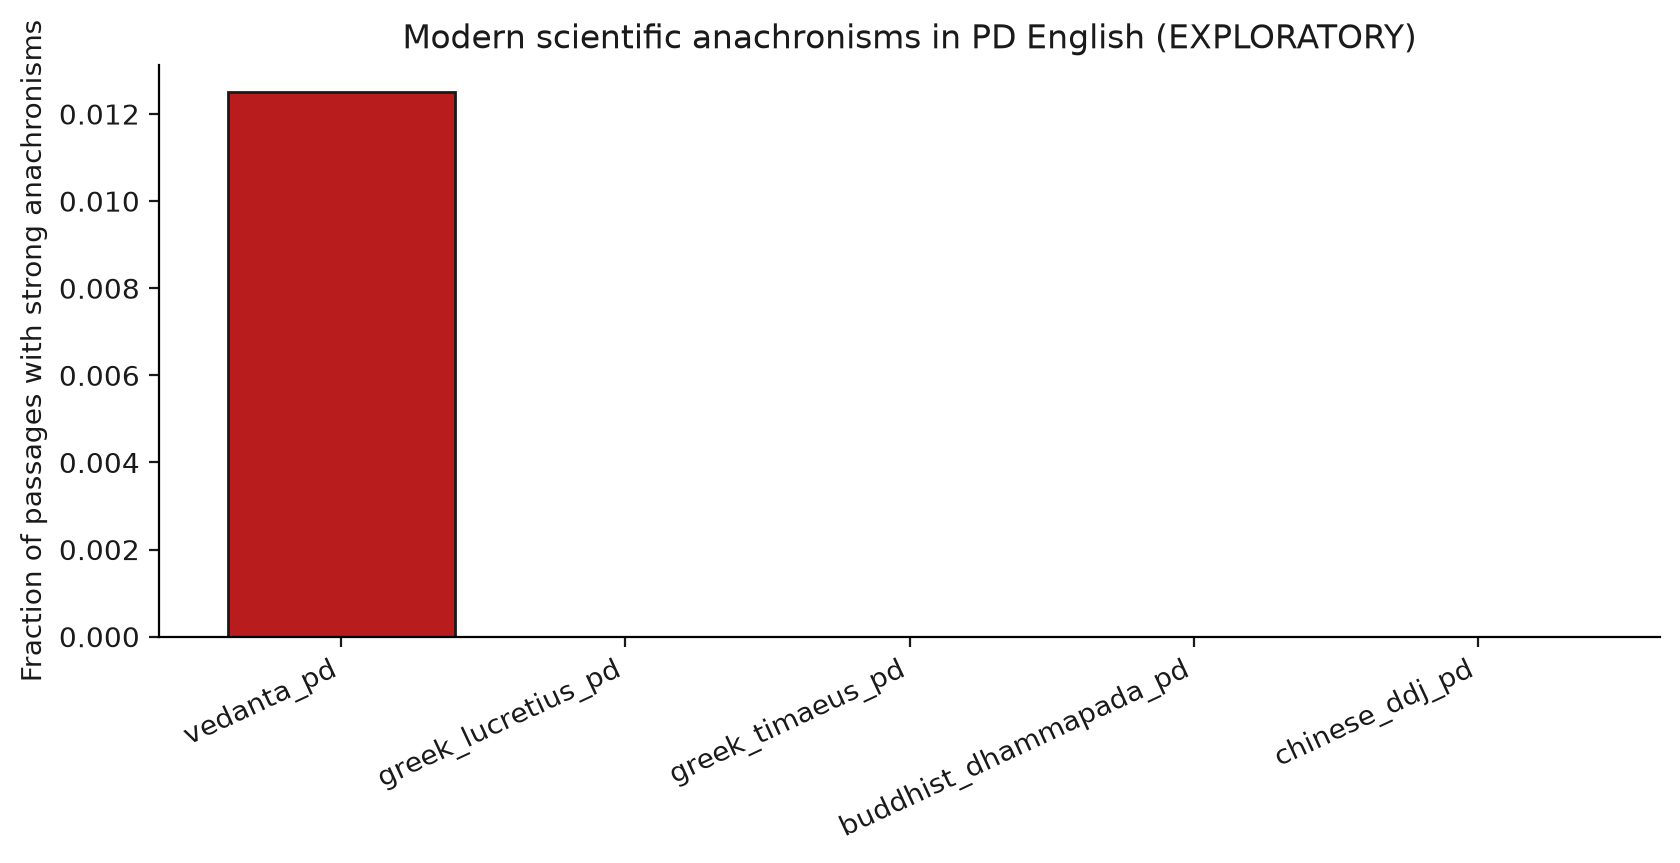
\includegraphics[width=\linewidth]{figures/fig32_contamination_by_tradition.png}
\caption{Strong modern-science anachronisms by tradition (EXPLORATORY).}
\label{fig:contam}
\end{figure}
\begin{figure}[H]
\centering
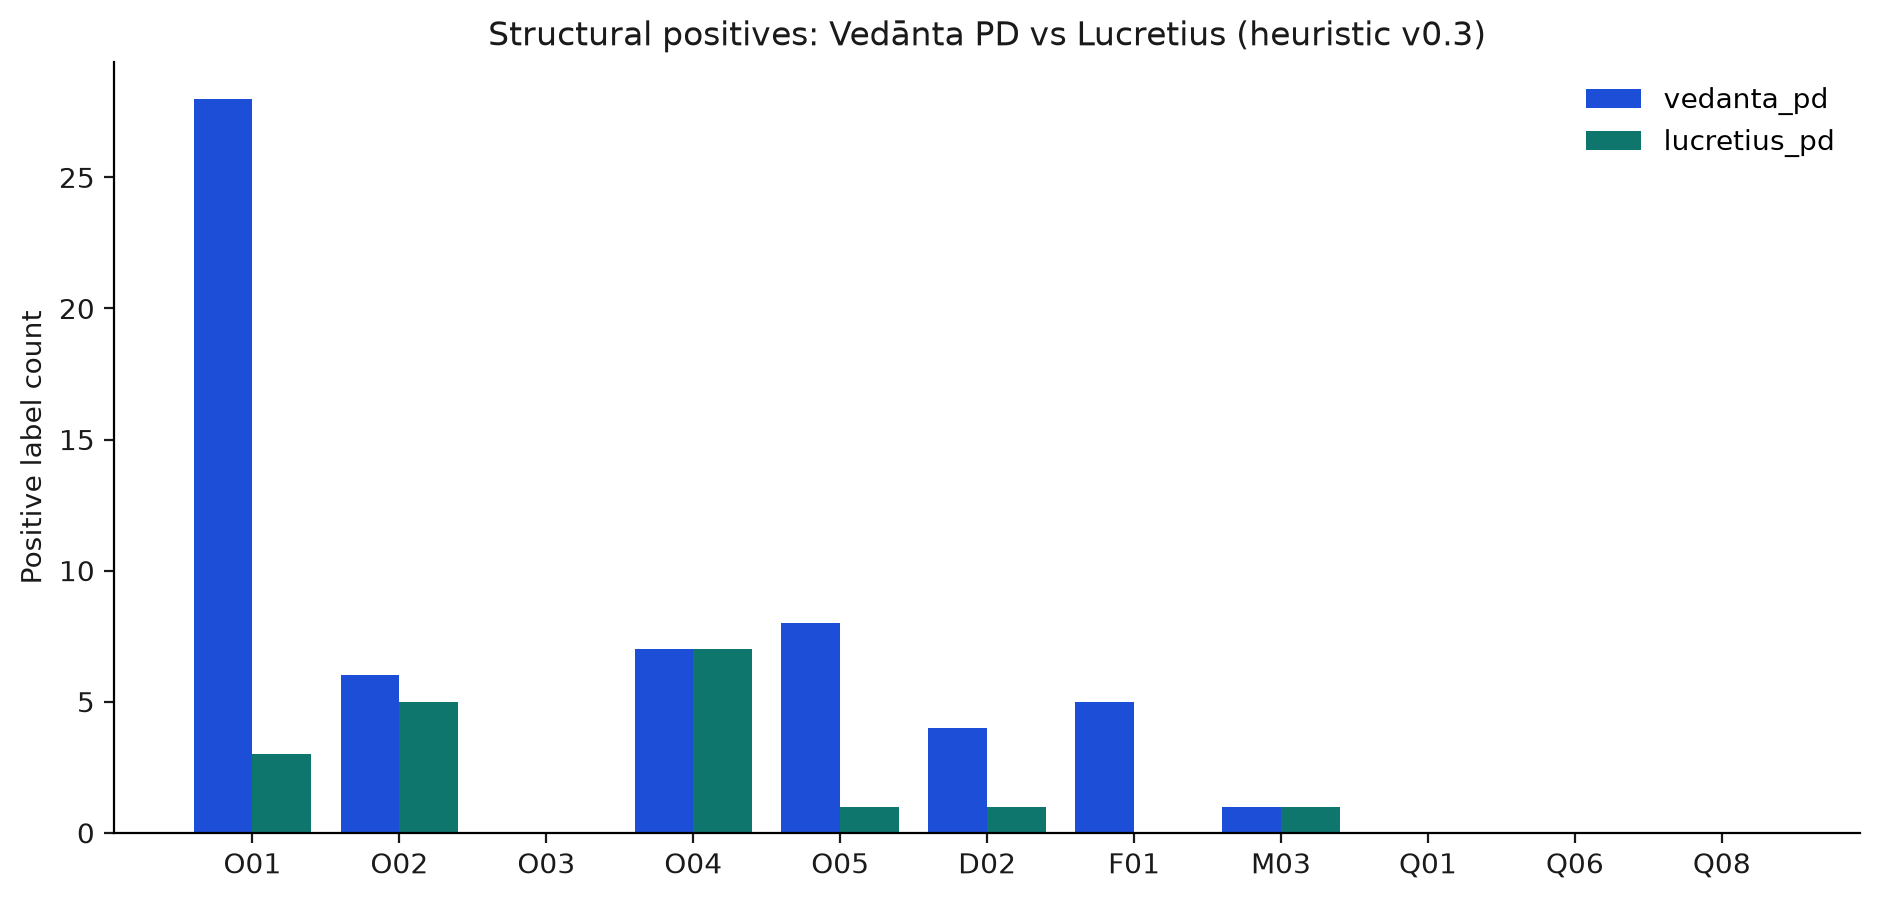
\includegraphics[width=\linewidth]{figures/fig33_vedanta_vs_lucretius_features.png}
\caption{Structural feature positives: Ved\={a}nta PD vs Lucretius (heuristic v0.3).}
\label{fig:vl}
\end{figure}
\begin{figure}[H]
\centering
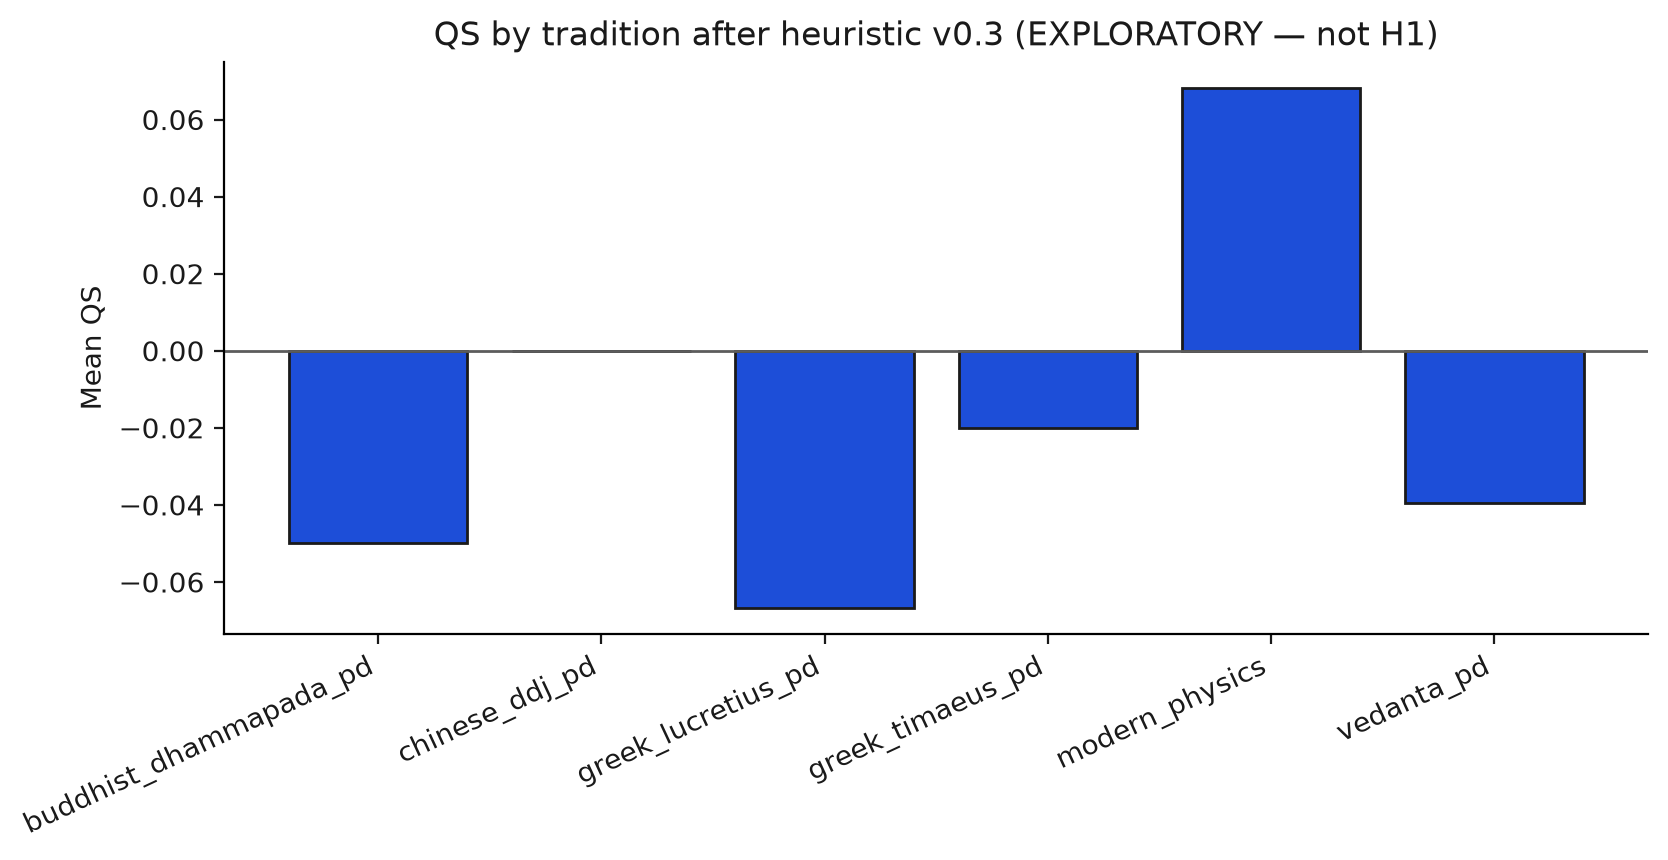
\includegraphics[width=0.92\linewidth]{figures/fig34_qs_after_v03.png}
\caption{QS by tradition after heuristic v0.3 (EXPLORATORY --- not confirmatory H1).}
\label{fig:qsv3}
\end{figure}
This triad is a Tier~2 quantitative finding about \emph{how} quantum--Sanskrit rhetoric mixes metaphysics, classical analogies, and modern editorial vocabulary---not a Tier~5 ancient-discovery claim.

\section{Exploratory System~B Findings}
\subsection{Motifs and enrichment}
\begin{figure}[H]
\centering
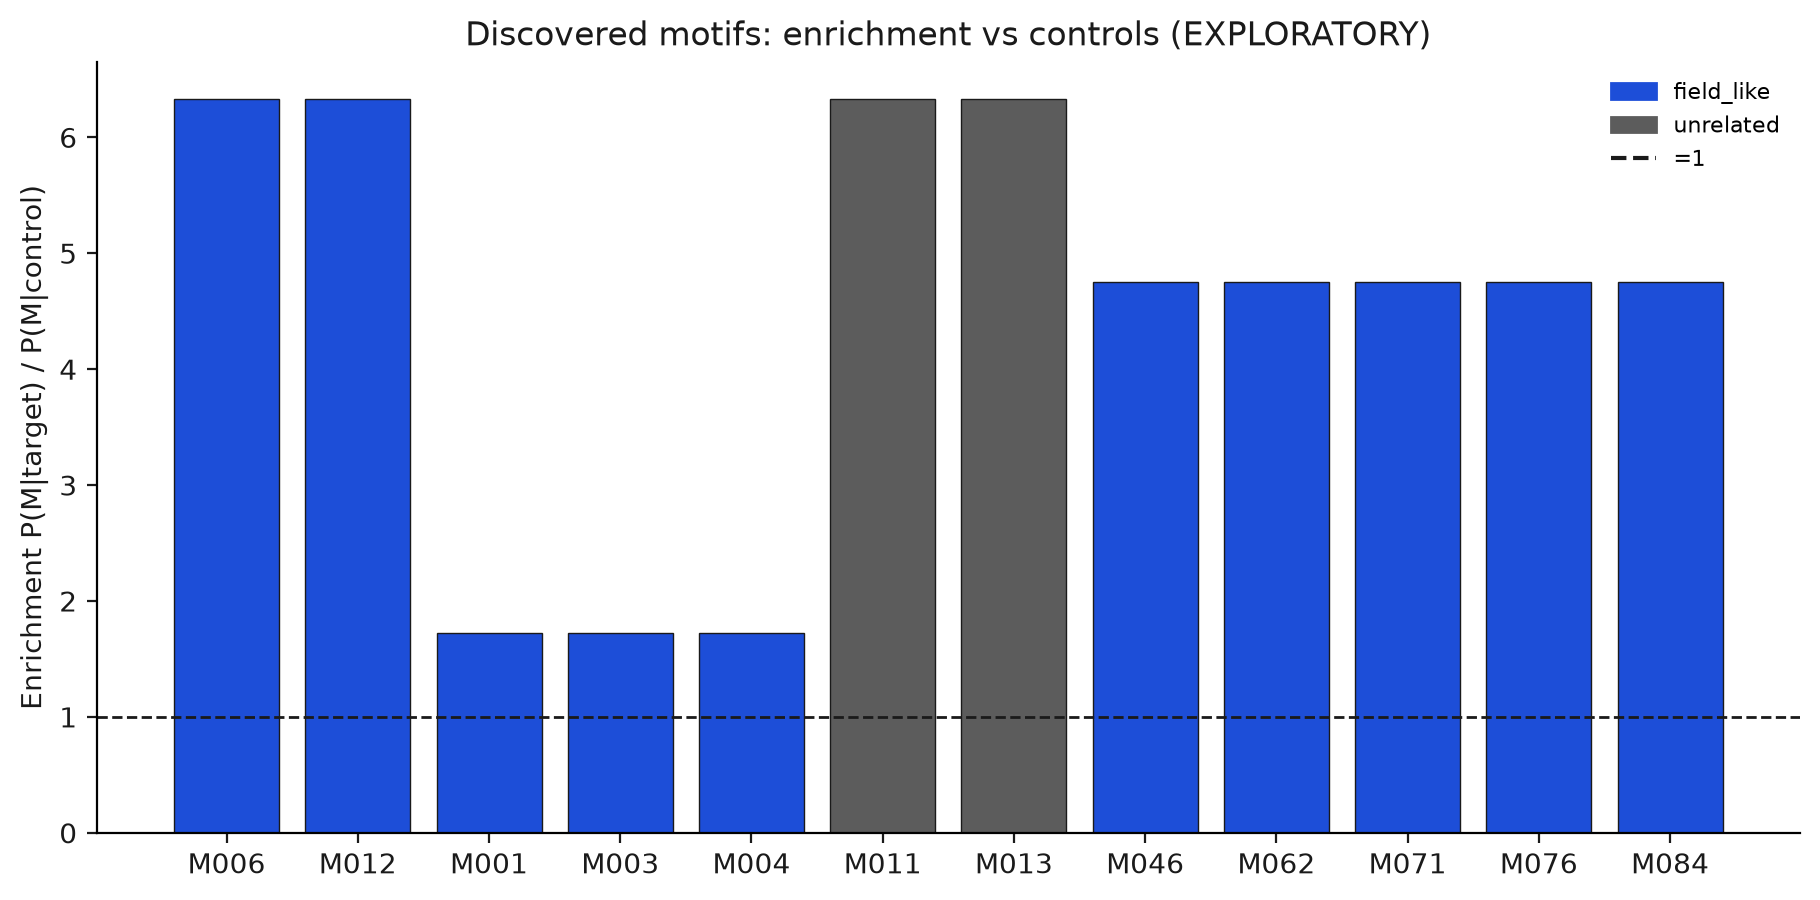
\includegraphics[width=\linewidth]{figures/fig20_discovery_motif_enrichment.png}
\caption{Top discovered motifs with post-hoc physics families (EXPLORATORY).}
\label{fig:motifenr}
\end{figure}
\begin{figure}[H]
\centering
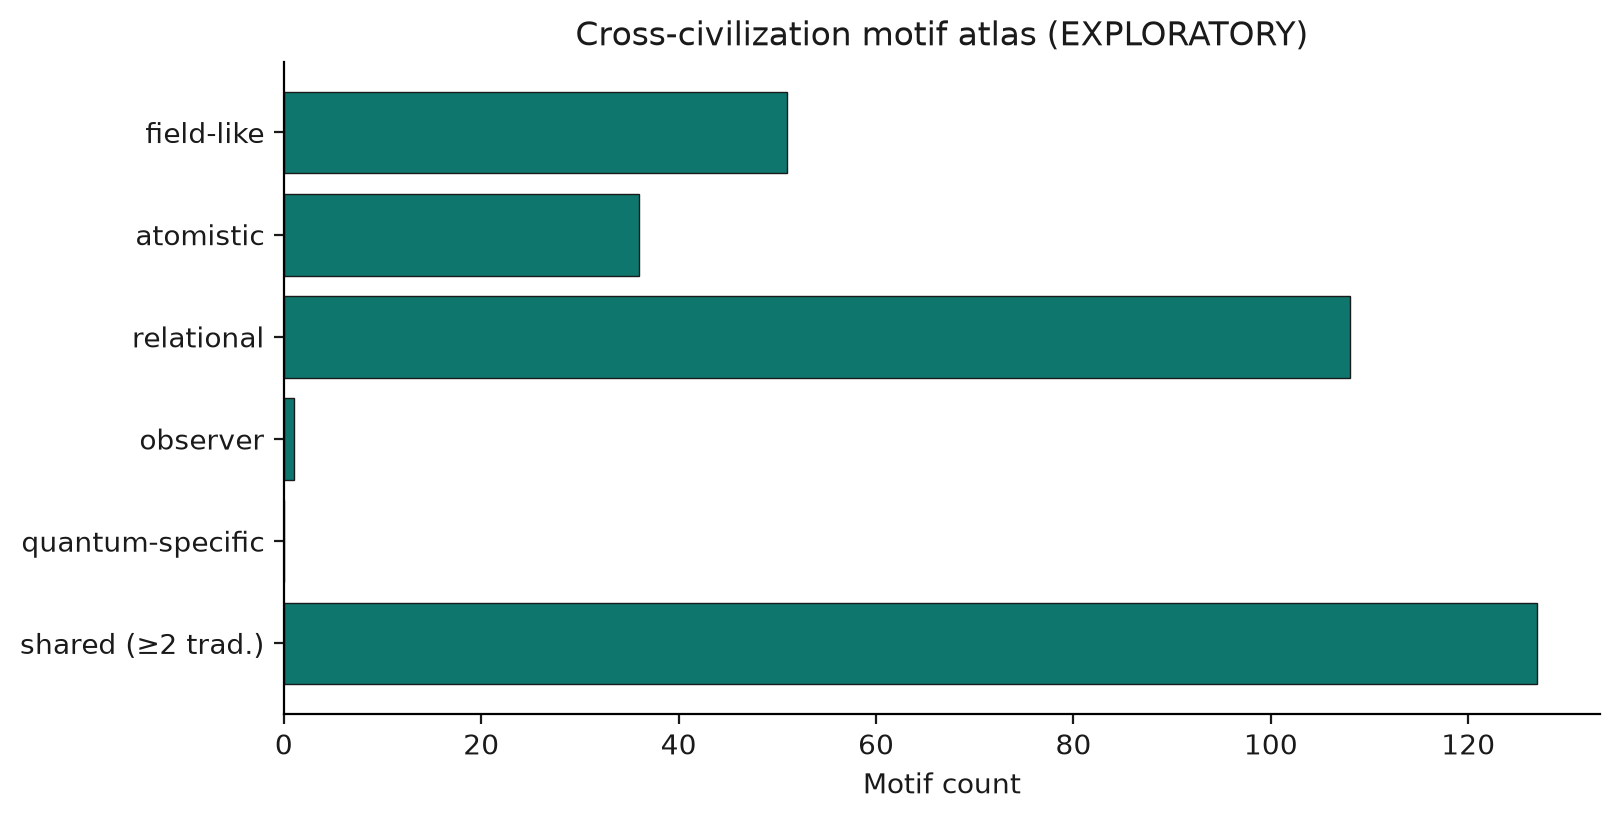
\includegraphics[width=\linewidth]{figures/fig21_discovery_motif_atlas.png}
\caption{Cross-civilization motif atlas categories.}
\label{fig:atlas}
\end{figure}
\begin{figure}[H]
\centering
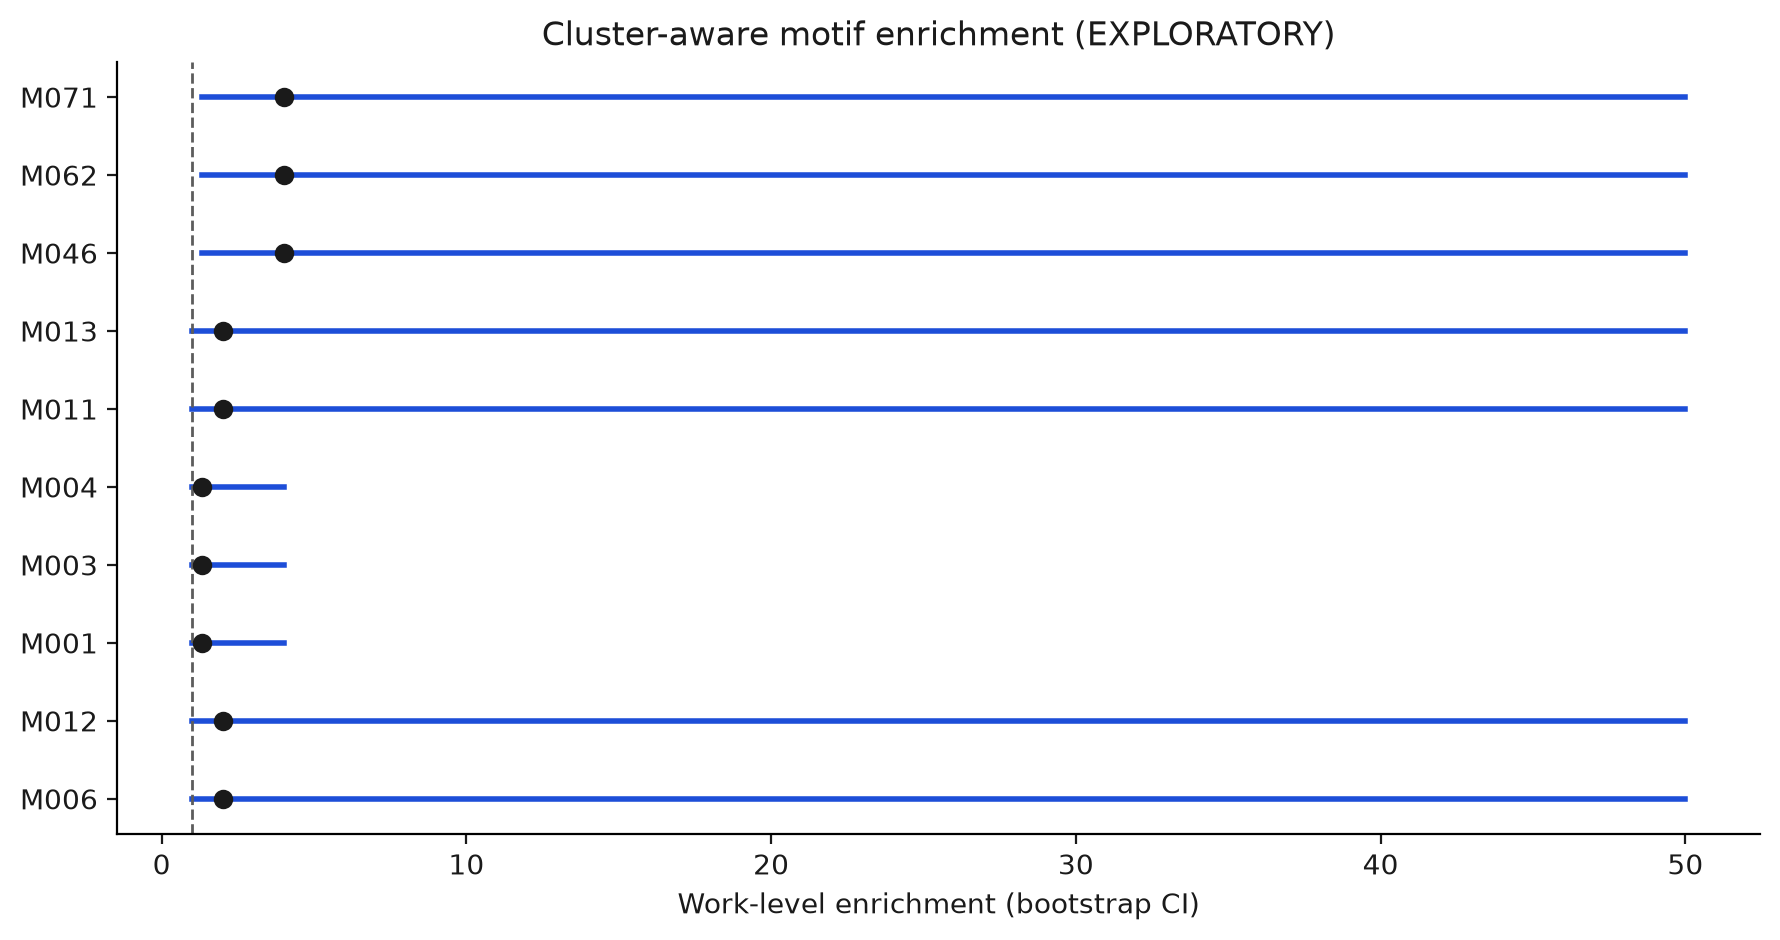
\includegraphics[width=\linewidth]{figures/fig30_cluster_bootstrap.png}
\caption{Work-cluster bootstrap enrichment intervals for top motifs.}
\label{fig:cluster}
\end{figure}
Under the heuristic PD annotations, \textbf{no quantum-specific motifs} were identified.
Several field-like motifs appear preferentially in historical \emph{controls} rather than the Sanskrit target slice---a claim-weakening pattern for Sanskrit-specific quantum readings of those structures.

\subsection{Surprisal, temporal, translation}
\begin{figure}[H]
\centering
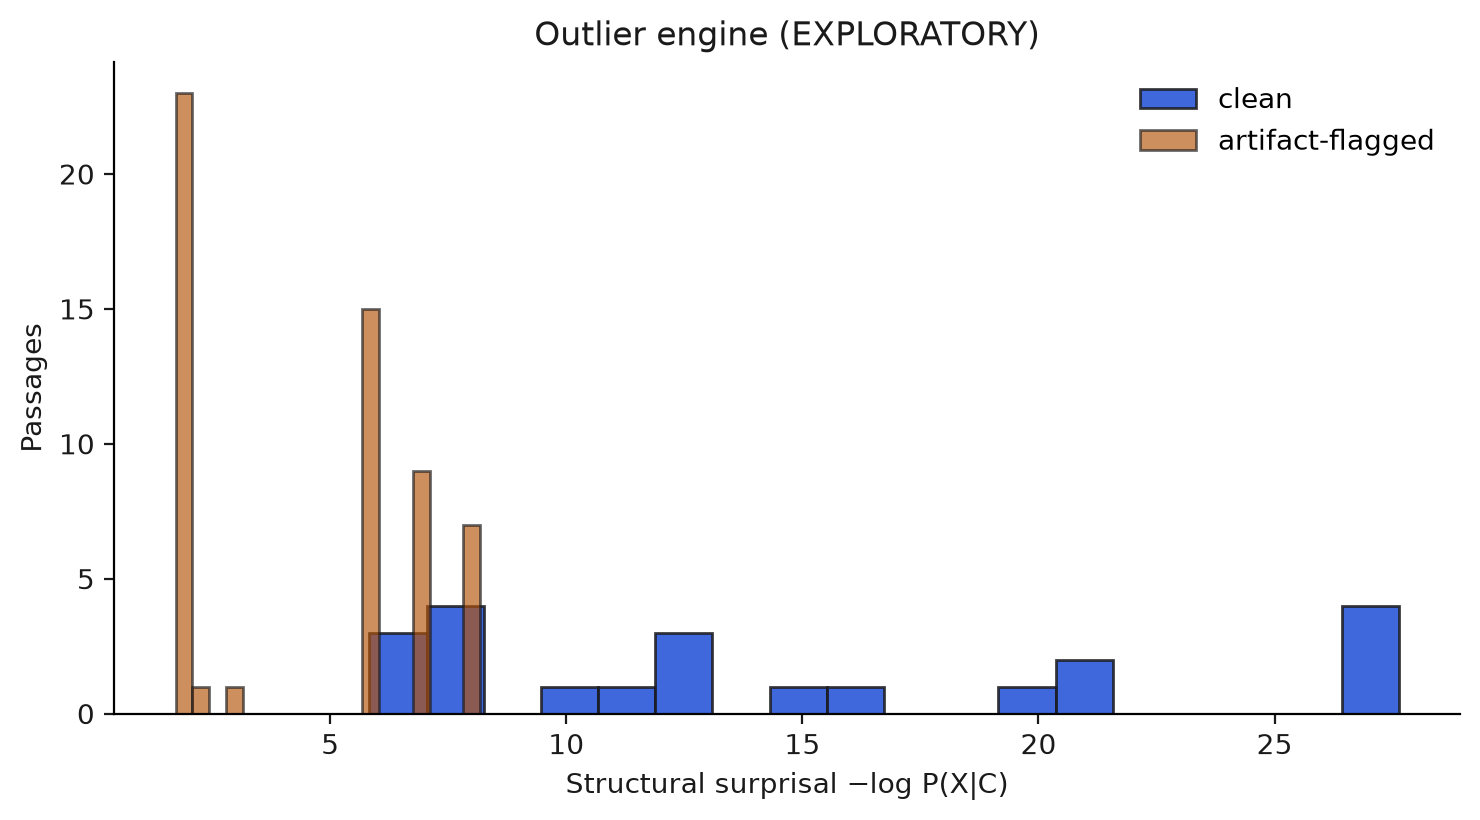
\includegraphics[width=0.9\linewidth]{figures/fig22_discovery_surprisal.png}
\caption{Structural surprisal with artifact flags.}
\label{fig:surprisal}
\end{figure}
\begin{figure}[H]
\centering
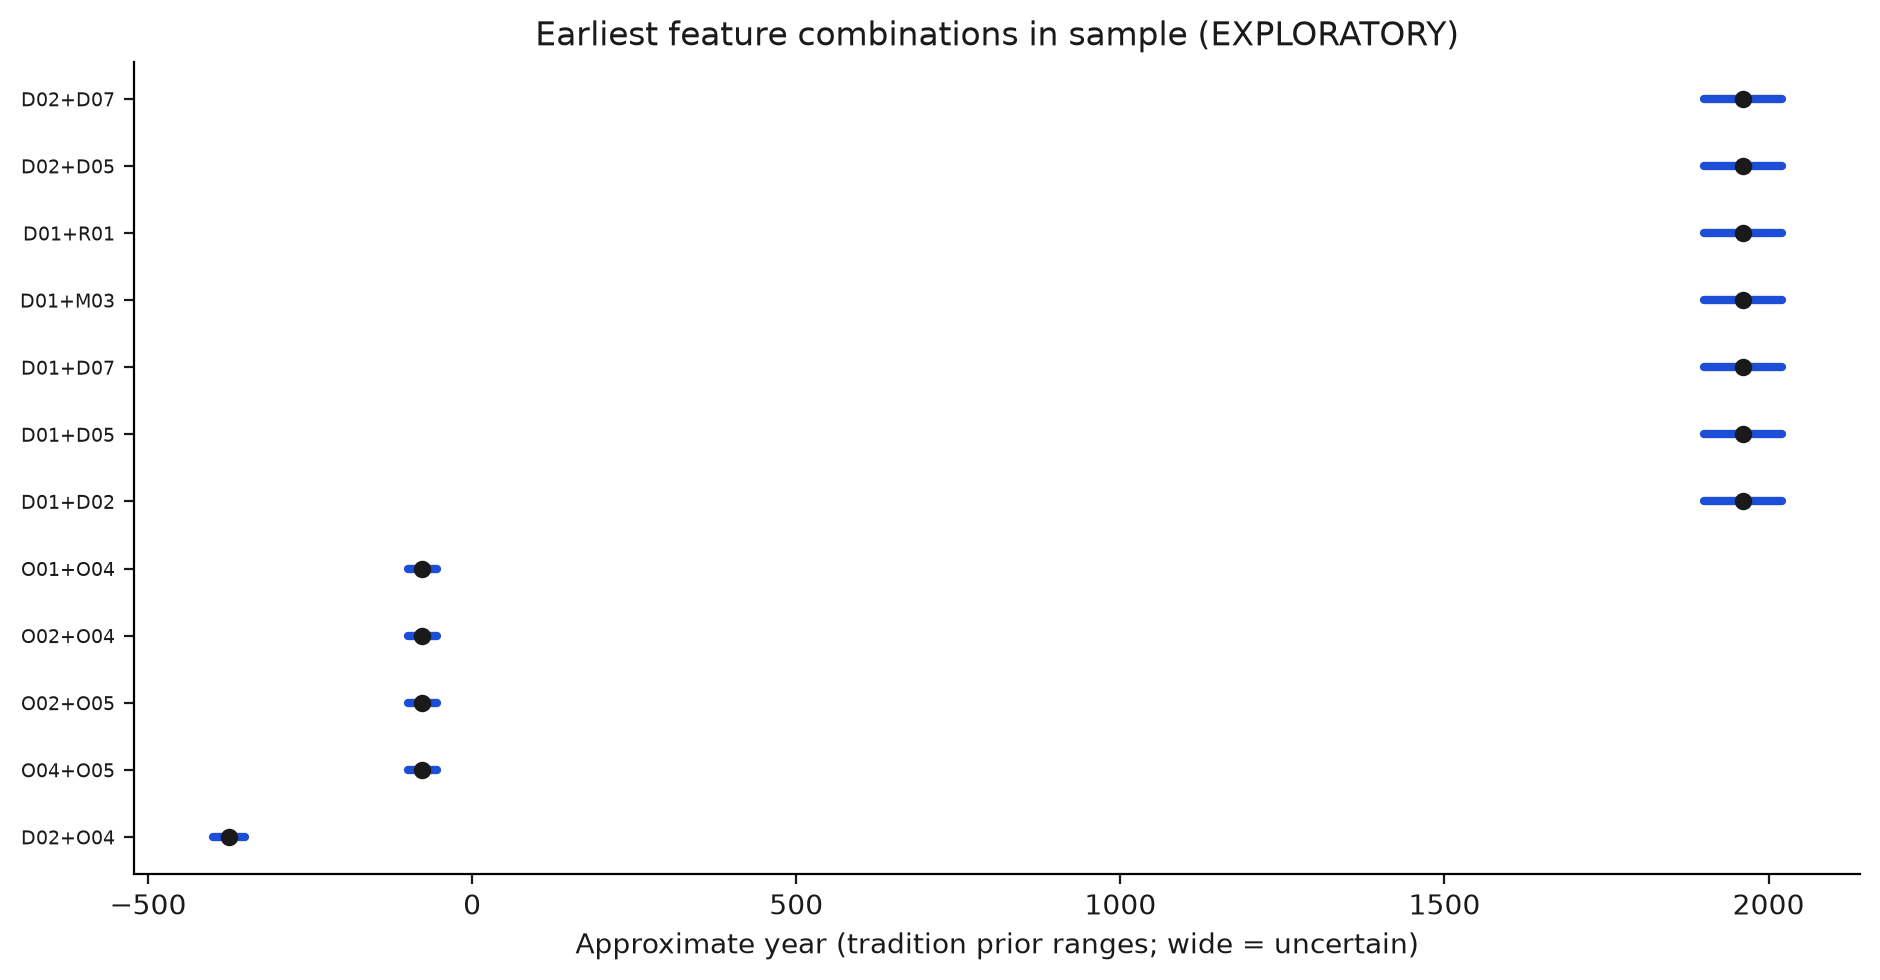
\includegraphics[width=\linewidth]{figures/fig28_temporal_combinations.png}
\caption{Earliest feature combinations using wide tradition date priors.}
\label{fig:temporal}
\end{figure}
\begin{figure}[H]
\centering
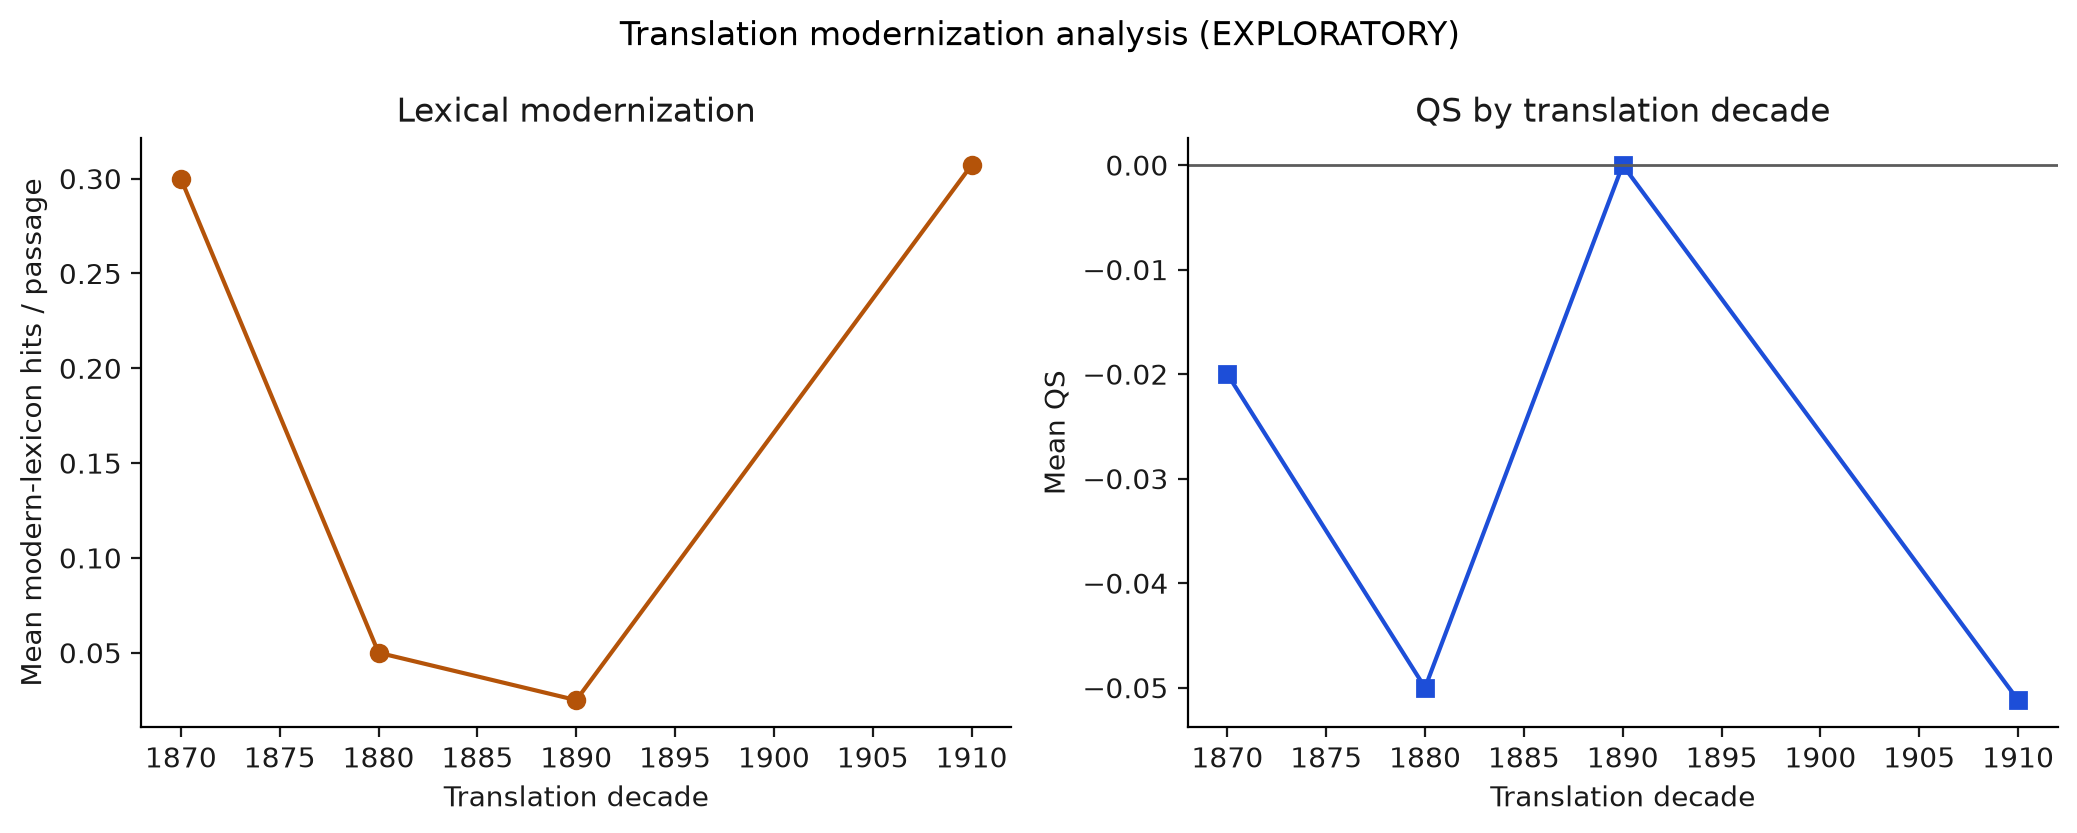
\includegraphics[width=\linewidth]{figures/fig29_translation_modernization.png}
\caption{Lexical modernization vs QS by translation decade (exploratory).}
\label{fig:modlex}
\end{figure}
\begin{figure}[H]
\centering
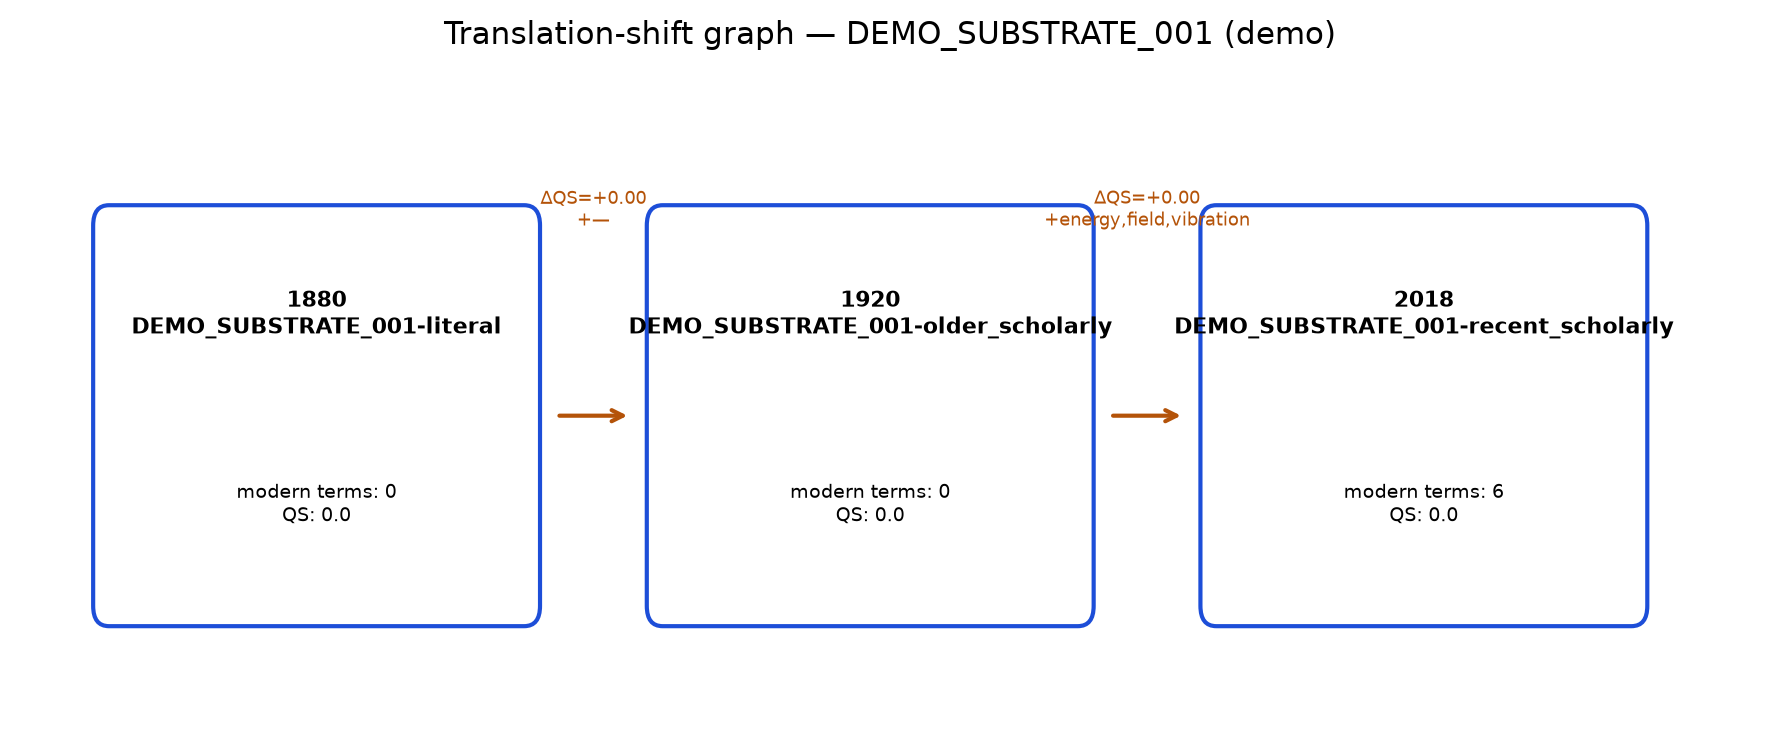
\includegraphics[width=\linewidth]{figures/fig31_translation_shift_graph.png}
\caption{Aligned translation-shift graph (synthetic multi-translation demo).}
\label{fig:shift}
\end{figure}
Synthetic translation demo: injecting ``quantum/energy/field/vibration'' wording yielded $\mathrm{TCI}\approx 0$ (Figure~\ref{fig:tci}).
\begin{figure}[H]
\centering
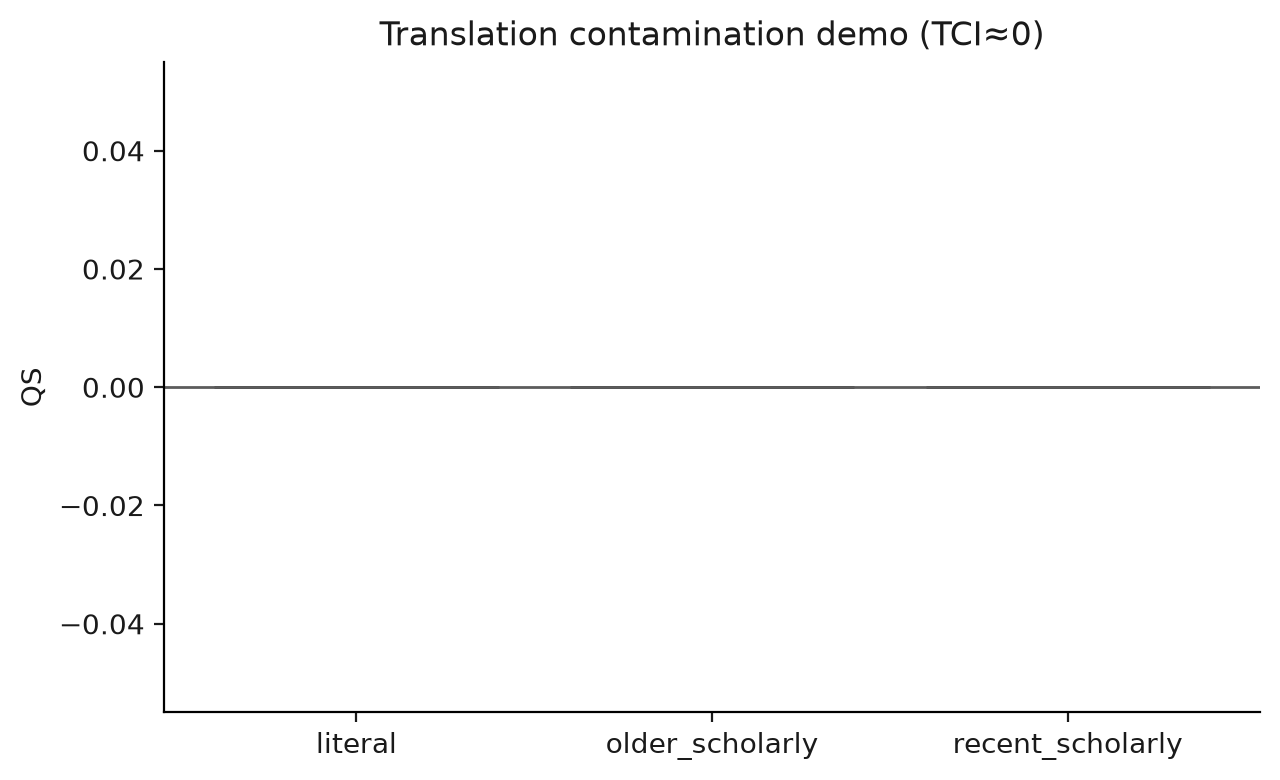
\includegraphics[width=0.75\linewidth]{figures/fig12_translation_tci_demo.png}
\caption{Synthetic translation-contamination demo.}
\label{fig:tci}
\end{figure}

\subsection{Claims vs data}
\begin{figure}[H]
\centering
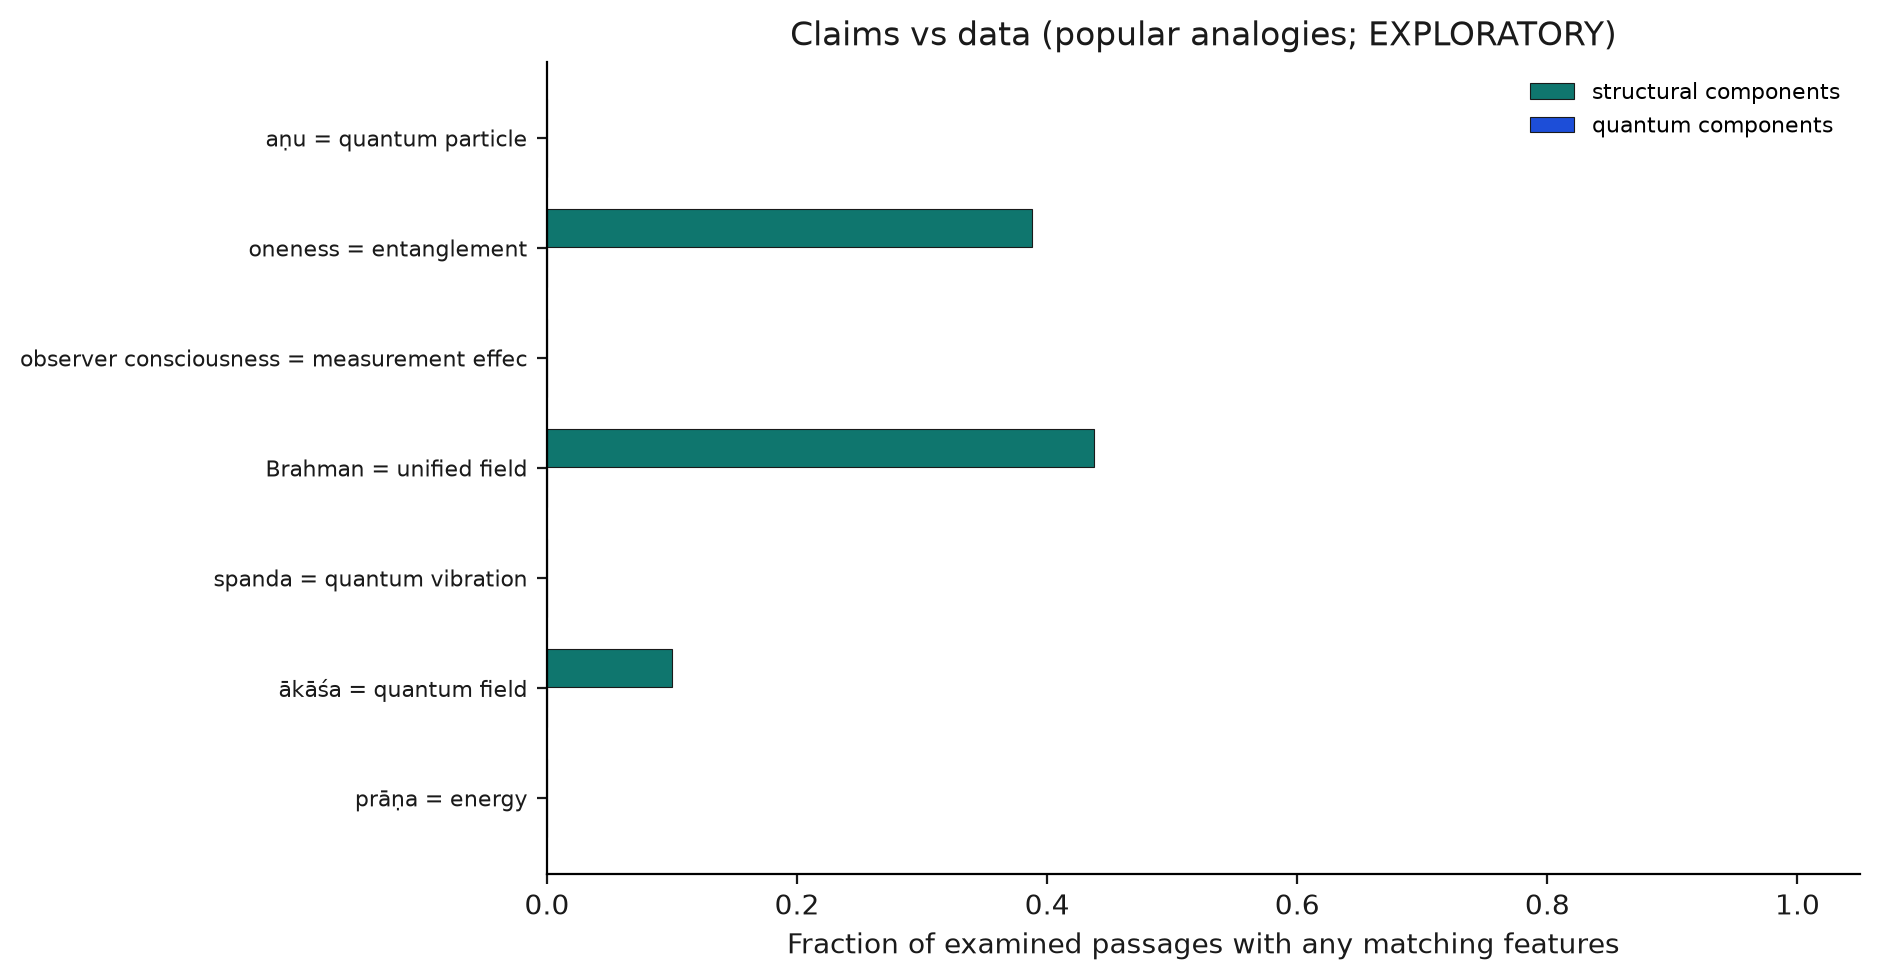
\includegraphics[width=\linewidth]{figures/fig27_claims_vs_data.png}
\caption{Popular claim components vs quantum components on Ved\={a}nta PD slice.}
\label{fig:claims}
\end{figure}
Popular quantum analogies are tested as structured claims.
Field-like support without Level~III features is reported as classical/field-like match---not as quantum confirmation and not as failure.

\subsection{Novelty gating}
No candidate was promoted to \texttt{STRONG\_DISCOVERY\_CANDIDATE}.
Automated literature search leaves all top motifs at \texttt{NOVELTY\_REVIEW\_REQUIRED}.
We do not claim ``first ever.''

\section{Robustness}
\begin{figure}[H]
\centering
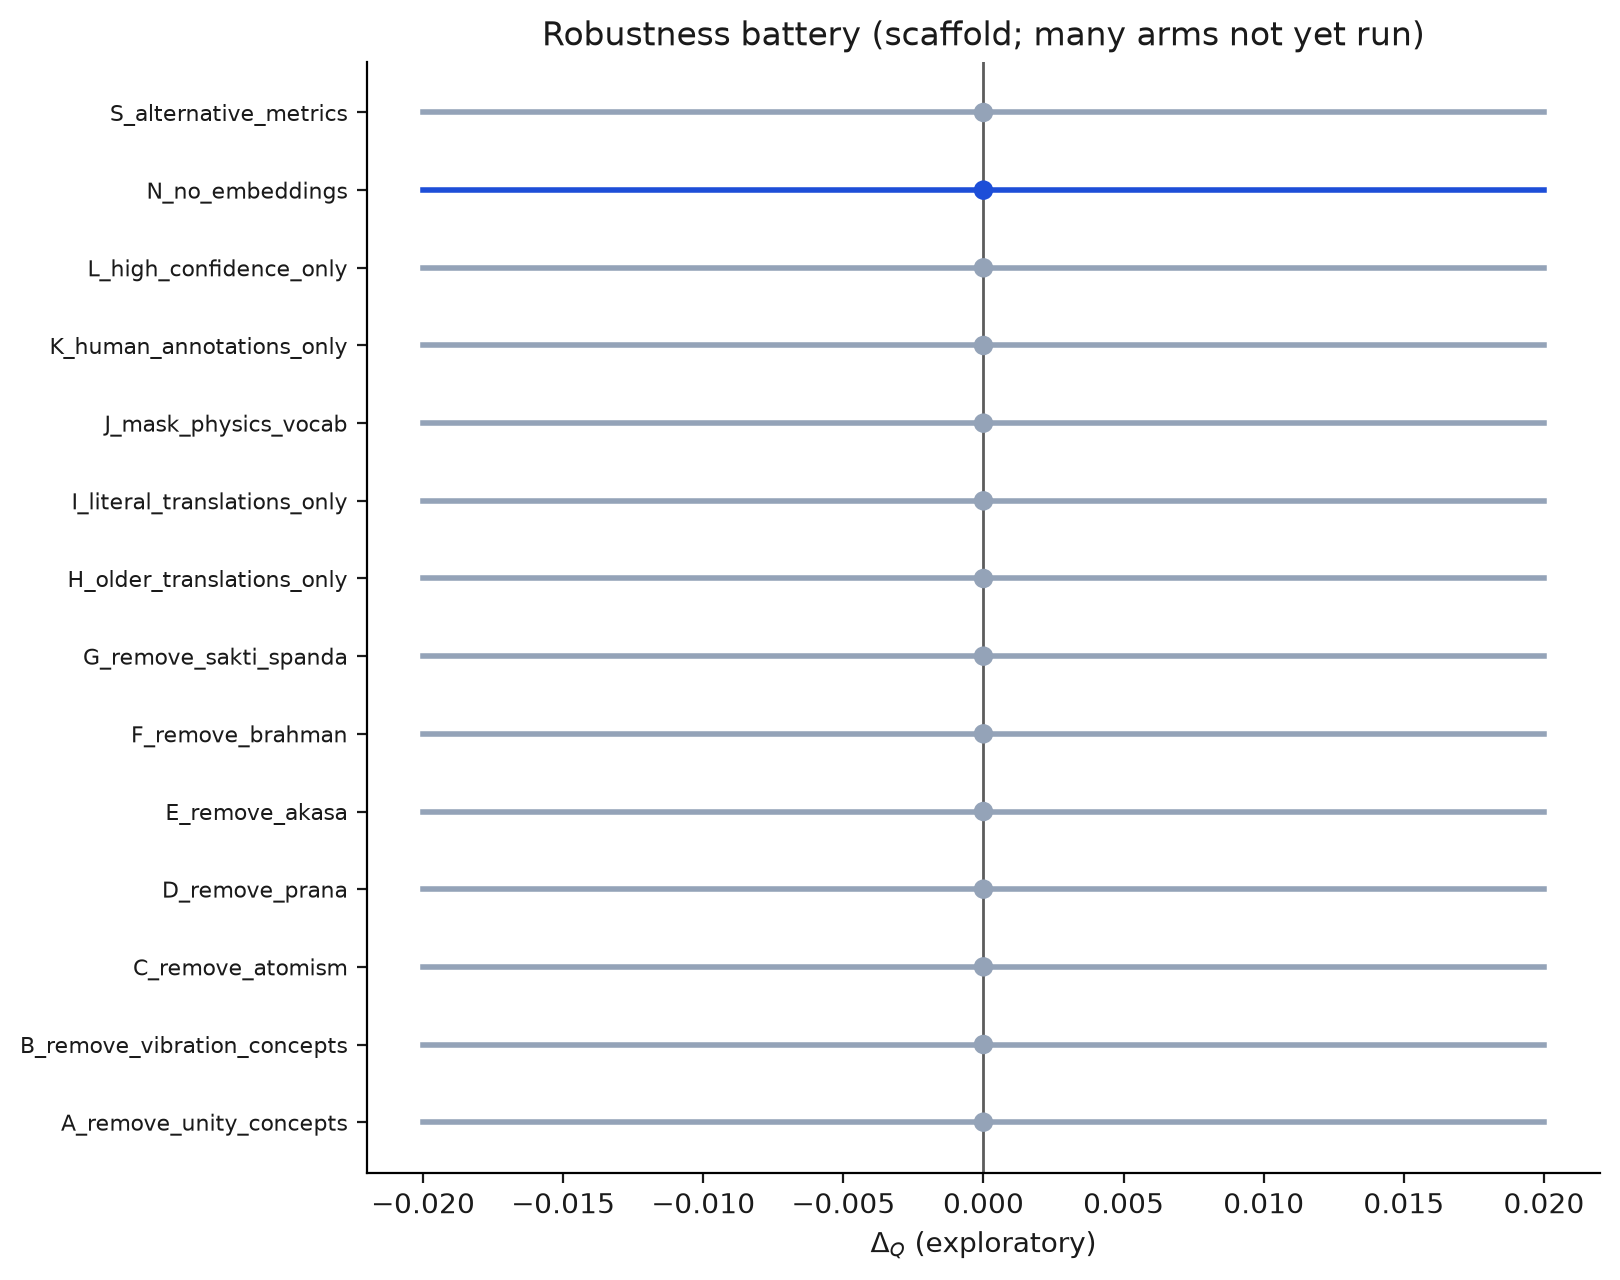
\includegraphics[width=0.9\linewidth]{figures/fig10_robustness_forest.png}
\caption{Robustness battery scaffold.}
\label{fig:robust}
\end{figure}

\section{Discussion}
\subsection{What is established so far}
\begin{enumerate}[leftmargin=*]
\item The ontology distinguishes classical fields from quantized fields and unity from nonseparability on controls.
\item A dual confirmatory/discovery architecture is implemented with an explicit novelty gate.
\item Under heuristic PD annotation, System~B finds field-like/compositional structure without quantum-specific motif enrichment for the Sanskrit target slice.
\end{enumerate}

\subsection{What remains}
Freeze ontology after further piloting; licensed multi-translation pairs; human validation; expert review; OSF preregistration; LLM annotation; confirmatory unlock once.

\subsection{Interpretation ladder}
Textual similarity $\rightarrow$ structural analogy $\rightarrow$ statistical enrichment $\rightarrow$ quantum-vs-classical specificity $\rightarrow$ multiple independent Level~III features.
Even the top rung is not historical discovery of QM.

\section{Limitations}
Heuristic annotators are brittle; PD English is not a substitute for philologically controlled Sanskrit editions; dating uses wide priors; development decisions contaminate exploratory data; novelty search is automated and incomplete.
See \texttt{docs/LIMITATIONS.md}.

\section{Conclusion}
RISHI-Q is both a confirmatory instrument and a discovery engine.
The present manuscript freezes the methodological story, demonstrates instrument behavior on controls, and reports exploratory System~B outputs without manufacturing significance.
Confirmatory evaluation remains locked until preregistration and human validation are complete.
\textbf{Rigor first; discovery second; extraordinary claims only with extraordinary evidence.}

\section*{Data and code availability}
Software: MIT-licensed repository.
Regenerate exhibits:
\begin{verbatim}
uv run python scripts/run_discovery_engine.py
uv run python scripts/build_all_visualizations.py
uv run python scripts/build_paper_assets.py
\end{verbatim}

\section*{Acknowledgments}
External Sanskrit, physics, and statistics reviewers are invited; none are invented here.

\bibliographystyle{plain}
\bibliography{references}

\appendix
\section{Ontology feature inventory}
% Auto-generated — do not edit by hand
% Generated: 2026-08-15T18:05:51.958695+00:00
\begin{table}[t]
\centering
\caption{RISHI-Q ontology v0.1 feature inventory.}
\label{tab:ontology-features}
\begin{tabular}{llllll}
\toprule
id & name & family & level & quantum\_specific & field\_like \\
\midrule
O01 & Fundamental substrate & fundamental\_ontology & I & False & False \\
O02 & Constituents & fundamental\_ontology & II & False & False \\
O03 & Fundamental discreteness & fundamental\_ontology & II & False & False \\
O04 & Continuous substrate & fundamental\_ontology & II & False & True \\
O05 & Local manifestation & fundamental\_ontology & II & False & True \\
O06 & Emergence & fundamental\_ontology & II & False & False \\
D01 & State & dynamics & II & False & False \\
D02 & Transformation & dynamics & II & False & False \\
D03 & Periodicity & dynamics & II & False & True \\
D04 & Propagation & dynamics & II & False & True \\
D05 & Conservation & dynamics & II & False & False \\
D06 & Symmetry & dynamics & II & False & False \\
D07 & Reversibility & dynamics & II & False & False \\
Q01 & Discrete allowed states & quantum\_specific & III & True & False \\
Q02 & Superposed possibilities & quantum\_specific & III & True & False \\
Q03 & Fundamental probability & quantum\_specific & III & True & False \\
Q04 & Measurement-conditioned outcome & quantum\_specific & III & True & False \\
Q05 & Incompatible observables & quantum\_specific & III & True & False \\
Q06 & Nonseparability & quantum\_specific & III & True & False \\
Q07 & Context dependence & quantum\_specific & III & True & False \\
Q08 & Quantized excitation & quantum\_specific & III & True & True \\
R01 & Local causation & relational & II & False & True \\
R02 & Long-range relation & relational & II & False & False \\
R03 & Holistic state & relational & II & False & False \\
R04 & Relational properties & relational & II & False & False \\
M01 & Observer/system distinction & observer\_epistemic & II & False & False \\
M02 & Observation modifies system & observer\_epistemic & III & True & False \\
M03 & Epistemic limitation & observer\_epistemic & I & False & False \\
M04 & Ontic indeterminacy & observer\_epistemic & III & True & False \\
F01 & Spatial distribution & field\_like & II & False & True \\
F02 & Local state of distributed entity & field\_like & II & False & True \\
F03 & Disturbance propagation & field\_like & II & False & True \\
F04 & Localized manifestation & field\_like & II & False & True \\
F05 & Interaction mediation & field\_like & II & False & True \\
F06 & Excitation-like structure & field\_like & II & False & True \\
F07 & Quantization of distributed structure & field\_like & III & True & True \\
\bottomrule
\end{tabular}
\end{table}

\section{Exploratory passage scores}
% Auto-generated — do not edit by hand
% Generated: 2026-08-15T18:05:51.915480+00:00
\begin{table}[t]
\centering
\caption{Exploratory passage scores (synthetic + physics controls). Not confirmatory.}
\label{tab:passage-scores}
\begin{tabular}{llllllllllll}
\toprule
passage\_id & tradition & role & QS & QEF & field\_class & newtonian & classical\_em & thermodynamics & relativity & quantum\_mechanics & quantum\_field\_theory \\
\midrule
PHYS\_NEWTON\_001 & modern\_physics & physics\_reference & -0.500 & 0.000 & insufficient & 1.000 & 0.667 & 0.667 & 0.500 & 0.333 & 0.500 \\
PHYS\_EM\_001 & modern\_physics & physics\_reference & -0.100 & 0.000 & classical\_field\_like & 0.000 & 1.000 & 0.000 & 0.000 & 0.000 & 0.900 \\
PHYS\_THERMO\_001 & modern\_physics & physics\_reference & -1.000 & 0.000 & insufficient & 1.000 & 0.500 & 1.000 & 0.000 & 0.000 & 0.000 \\
PHYS\_QM\_001 & modern\_physics & physics\_reference & 0.900 & 1.000 & insufficient & 0.000 & 0.000 & 0.000 & 0.100 & 1.000 & 0.333 \\
PHYS\_QFT\_001 & modern\_physics & physics\_reference & 0.333 & 1.000 & potentially\_qft\_like & 0.000 & 0.667 & 0.000 & 0.000 & 0.200 & 1.000 \\
PHYS\_ENTANGLE\_001 & modern\_physics & physics\_reference & 0.800 & 1.000 & insufficient & 0.000 & 0.000 & 0.000 & 0.000 & 0.800 & 0.500 \\
SYN\_UNITY\_001 & synthetic\_metaphysical & negative\_control & 0.000 & 0.000 & insufficient & 0.000 & 0.000 & 0.000 & 0.000 & 0.000 & 0.000 \\
SYN\_FIELD\_001 & synthetic\_target\_like & target & 0.000 & 0.000 & metaphor\_substrate\_only & 0.000 & 0.750 & 0.000 & 0.000 & 0.000 & 0.750 \\
SYN\_ATOM\_001 & synthetic\_vaisheshika\_like & target & -0.333 & 0.000 & insufficient & 0.667 & 0.333 & 0.000 & 0.333 & 0.333 & 0.333 \\
SYN\_MYSTICAL\_001 & synthetic\_mystical & control & 0.000 & 0.000 & insufficient & 0.000 & 0.000 & 0.000 & 0.000 & 0.000 & 0.000 \\
SYN\_GREEK\_001 & greek & control & -0.333 & 0.000 & insufficient & 0.667 & 0.333 & 0.000 & 0.333 & 0.333 & 0.333 \\
\bottomrule
\end{tabular}
\end{table}

\section{Frequent positive features}
% Auto-generated — do not edit by hand
% Generated: 2026-08-15T18:05:51.927129+00:00
\begin{table}[t]
\centering
\caption{Most frequent positive ontology features in the exploratory run.}
\label{tab:positive-features}
\begin{tabular}{ll}
\toprule
feature\_id & n\_positive \\
\midrule
O04 & 3 \\
R01 & 3 \\
D04 & 3 \\
Q03 & 3 \\
O05 & 2 \\
O03 & 2 \\
O02 & 2 \\
M03 & 2 \\
Q06 & 2 \\
F05 & 2 \\
F04 & 2 \\
F03 & 2 \\
F01 & 2 \\
D05 & 2 \\
Q05 & 1 \\
Q04 & 1 \\
Q07 & 1 \\
Q02 & 1 \\
Q01 & 1 \\
Q08 & 1 \\
D01 & 1 \\
M04 & 1 \\
O01 & 1 \\
D02 & 1 \\
M02 & 1 \\
\bottomrule
\end{tabular}
\end{table}


\end{document}
